\chapter{RESULTADOS E DISCUSSÃO}
% Version passo 0.005
% 'Sim ref'	'2.94'	49
% 'Sim 1A'	'2.95'	49
% 'Sim 1B'	'0.74'	49
% 'Sim 2A'	'5.43'	49
% 'Sim 2B'	'0.88'	49
% 'Sim 3A'	'4.30'	81
% 'Sim 3B'	'1.52'	45
% 'Sim 4A'	'0.22'	25
% 'Sim 4B'	'93.02'	241
% 'Sim 5A'	'4.98'	85
% 'Sim 5B'	'1.50'	37
Este capítulo detalha os resultados alcançados por meio da simulação computacional do método de controle de trajetória proposto pelo presente trabalho. É apresentado a sequência de movimentos a serem simulados, assim como os parâmetros da simulação. Além disso, são realizadas as simulações com variações dos valores destes parâmetros para uma análise da influência dos mesmos nos resultados. É utilizado também o algoritmo Runge-Kutta para simular a trajetória percorrida pela ponta da impressora dada a trajetória da base, fornecendo dados para se comparar a influência do método de controle de trajetória proposto.

\section{Simulação Computacional e Análise de Dados}

As simulações são realizadas a partir de dois movimentos lineares: um deslocamento de 10 milímetros no eixo x seguido de um movimento similar no eixo y, partindo da posição inicial (0,0) e em estado de repouso. A Figura \ref{fig:base_mov} ilustra estes movimentos.

\begin{figure}[H]
    \centering
    \caption{Movimento base}
    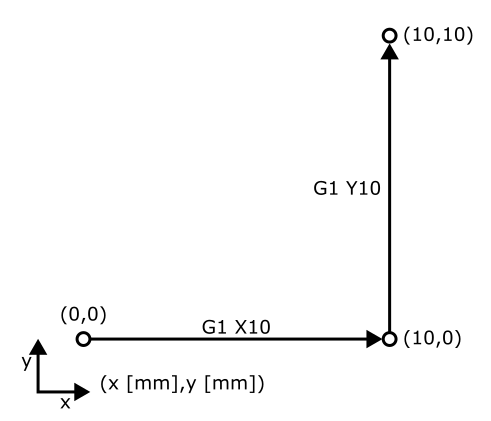
\includegraphics[scale=0.6]{base_mov}

    \label{fig:base_mov}
\end{figure}

Os parâmetros da simulação incluem a frequência natural e o coeficiente de amortecimento, responsáveis pela definição do modelo dinâmico da impressora. Adicionalmente, a aceleração e o passo de tempo são parâmetros que influenciam diretamente a trajetória, sendo estes definidos na fase de geração da mesma. Por fim, a velocidade estipulada no comando, que é parte integrante do Gcode, também é determinada. A origem e aplicação desses parâmetros são detalhadas na Figura \ref{fig:fluxo_geral_var}.

\begin{figure}[H]
    \centering
    \caption{Fluxograma geral com os parâmetros.}
    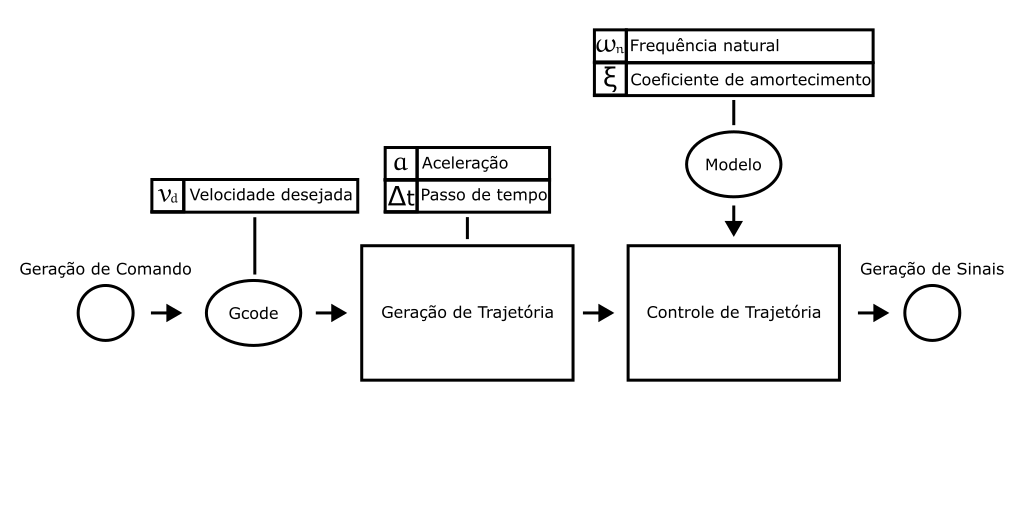
\includegraphics[scale=0.5]{fluxo_geral_var}

    \label{fig:fluxo_geral_var}
\end{figure}

As simulações foram executadas em um computador com as especificações listadas na Tabela \ref{tab:note_config}.

\begin{table}
    \begin{center}
    \caption{Especificações do computador}
    \label{tab:note_config}
    \begin{tabular}{c c}
        \hline
        Processador & Intel I7-5500U 2.40GHz \\
        Memoria & 8,00 GB \\
        Placa de vídeo & Nvidia Geforce 920M \\
        Sistema & 64 bits \\ \hline
    \end{tabular}
    \end{center}
\end{table}

\subsection{Simulação de Referência}
Nesta etapa, conduz-se uma simulação de referência empregando valores medianos dos parâmetros-chave. Esta simulação serve como base para avaliar o impacto de variações nos parâmetros em simulações subsequentes. Os valores referência utilizados são listados na Tabela \ref{tab:base_params}.

\begin{table}
    \begin{center}
    \caption{Valores dos parâmetros utilizados na simulação referência.}
    \label{tab:base_params}
    \begin{tabular}{c c c}
        Parâmetro & Valor & Unidade\\ \hline
        Frequência & 100 & $rad/s$\\
        Coeficiente de amortecimento & 0,5 & - \\
        Aceleração base & 5000 & $mm/s^2$ \\
        Passo de tempo & 0,005 & $s$ \\ 
        Velocidade desejada & 100 & $mm/s$ \\ \hline
    \end{tabular}
    \end{center}
\end{table}

\subsection{Simulações com Parâmetros Variados}
Para explorar o efeito de diferentes configurações, realizam-se simulações adicionais onde cada parâmetro - frequência natural, coeficiente de amortecimento, aceleração de entrada, passo de tempo e velocidade desejada - é variado individualmente. Estas variações incluem valores tanto inferiores quanto superiores aos da simulação de referência. No total, são 11 simulações: 10 delas dedicadas a testar os limites inferiores e superiores de cada parâmetro e uma utilizando os valores de referência. Os detalhes de cada simulação, incluindo a identificação numérica e a letra indicativa do parâmetro modificado (A para inferiores, B para superiores), são apresentados na Tabela \ref{tab:sim_params}.

\begin{table}
    \begin{center}
    \caption{Parâmetros utilizados nas simulações.}
    \label{tab:sim_params}
    \begin{tabular}{c c c c c}
        Caso & Parâmetro & Valor A & Valor B & Unidade\\ \hline
        1 & Frequência & 50 & 200 & $rad/s$\\
        2 & Coeficiente de amortecimento & 0 & 1 & - \\
        3 & Aceleração base & 1000 & 10000 & $mm/s^2$ \\
        4 & Passo de tempo & 0,1 & 0,001 & $s$ \\
        5 & Velocidade desejada & 50 & 200 & $mm/s$ \\ \hline
    \end{tabular}
    \end{center}
\end{table}

\subsection{Aplicação do método Runge-Kutta}
O controle de trajetória desenvolvido neste estudo, se da através da modificação da trajetória da base, com objetivo de diminuir o desvio do caminho da ponta em relação ao caminho desejado. Para poder avaliar se este objetivo está sendo cumprido se faz necessário a trajetória da ponta, considerando as características dinâmicas da impressora. Para isso foi aplicado o método Runge-Kutta na trajetória da base obtida pelo controle de trajetória, aplicou-se este método também na trajetória não modificada pelo controle de trajetória, representando o comportamento da impressora que não implementa esta etapa. Além disso, fez-se necessário a interpolação dos pontos da trajetória por conta de baixa precisão e até mesmo a incapacidade do método Runge-Kutta de gerar resultados confiáveis. Entretanto, a partir do momento em que aplicou-se a interpolação de um passo de tempo de 0.0001 segundos, os resultados se mostraram consistentes.

\section{Resultados das Simulações}
A análise dos resultados começa com a avaliação da simulação de referência, estabelecendo um ponto de partida para comparações. Posteriormente, a análise foca no impacto e nas consequências das alterações nos parâmetros. Este estudo inclui a variação dos elementos do modelo dinâmico da impressora, como frequência natural e coeficiente de amortecimento, seguido pela investigação das mudanças nos parâmetros relacionados à geração de trajetória, especificamente aceleração e passo de tempo. Além disso, examina-se a influência das variações no parâmetro de velocidade desejada do Gcode.

\subsection{Resultados da Simulação de Referência}
Esta seção apresenta uma análise detalhada dos resultados obtidos pela simulação de referência dispostos nos gráficos a seguir.

% ------------------ Caminho ----------------
O primeiro gráfico (Figura \ref{fig:}) ilustra o caminho da base no plano XY. Observa-se um movimento na direção X, inicialmente sobreposto ao caminho desejado. Entretanto, próximo a região de transição do movimento em X para o movimento em Y existe um arredondamento da curva ou uma antecipação do movimento em Y.
Os efeitos deste comportamento podem ser melhor avaliados na Figura \ref{fig:}, onde é apresentado os caminhos da ponta simulados para os caminhos da base com controle de trajetória e sem, assim como o caminho desejado.

% fig:cam
\begin{figure}[H]
    \centering
    \subfigure[Sem controle.]{
        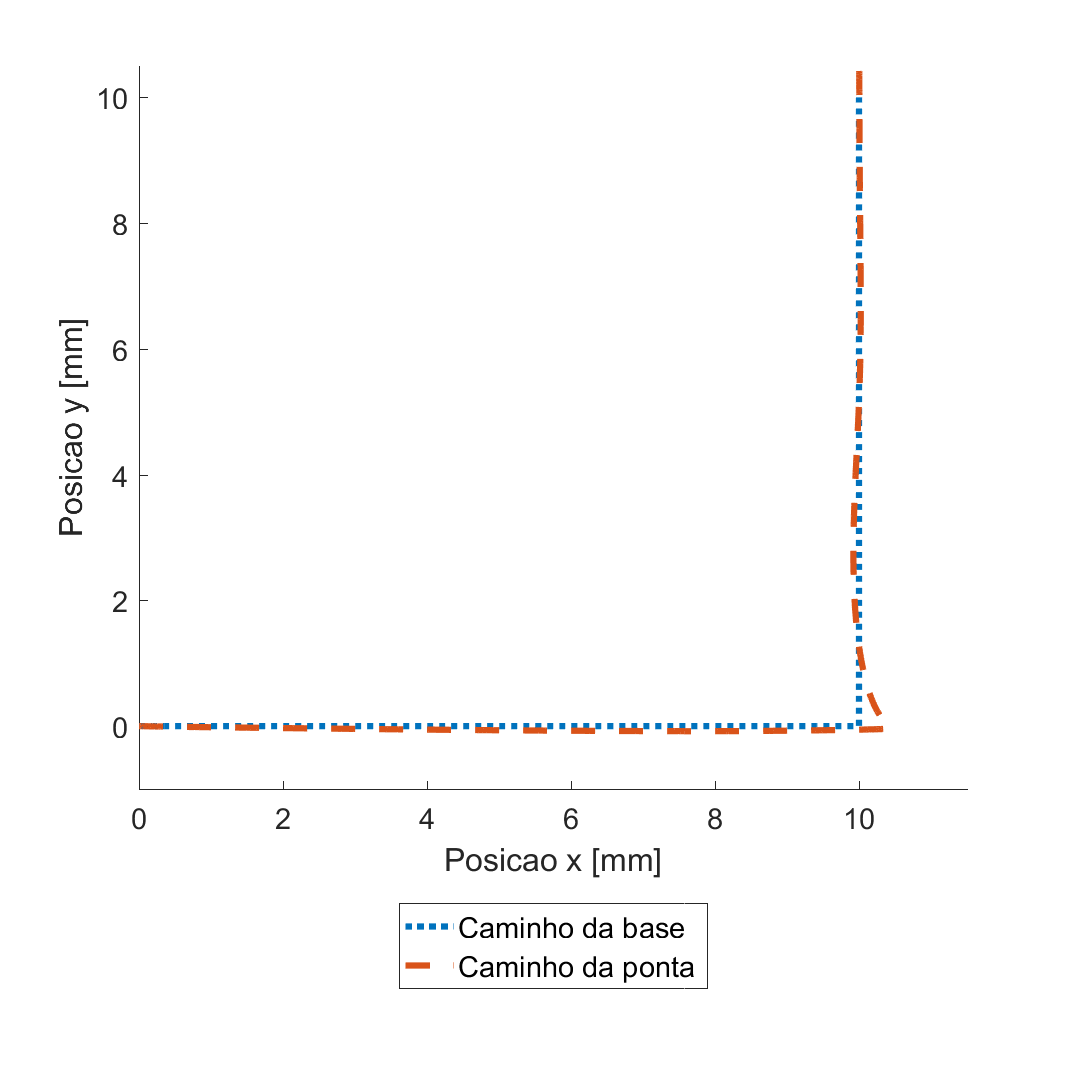
\includegraphics[width=0.47\textwidth]{Sim ref_cam_s.png}
        \label{fig:ref_cam_s}
    }
    \hfill
    \subfigure[Com controle.]{
        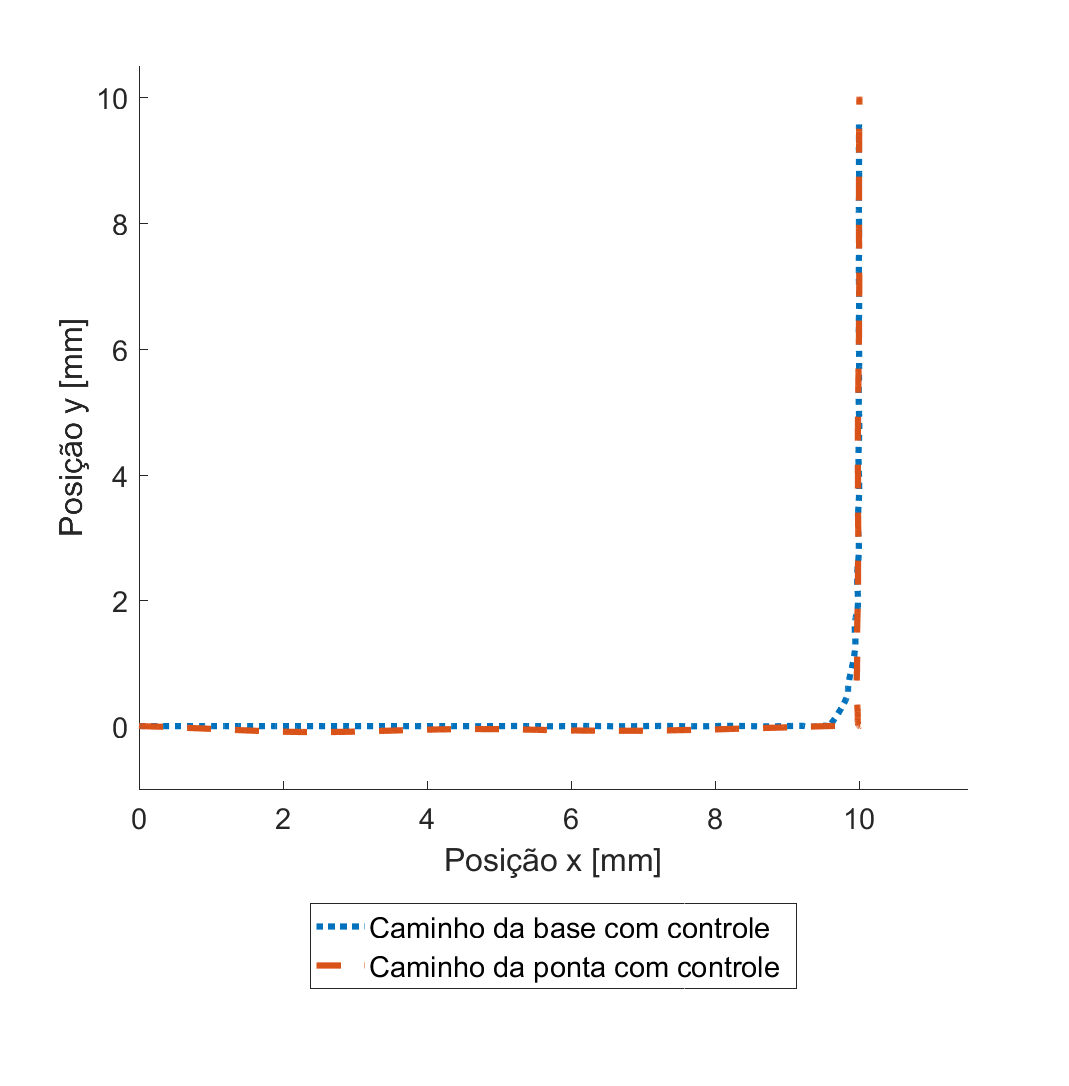
\includegraphics[width=0.47\textwidth]{Sim ref_cam_c.png}
        \label{fig:ref_cam_c}
    }
    \hfill
    \subfigure[Detalhamento - Sem controle.]{
        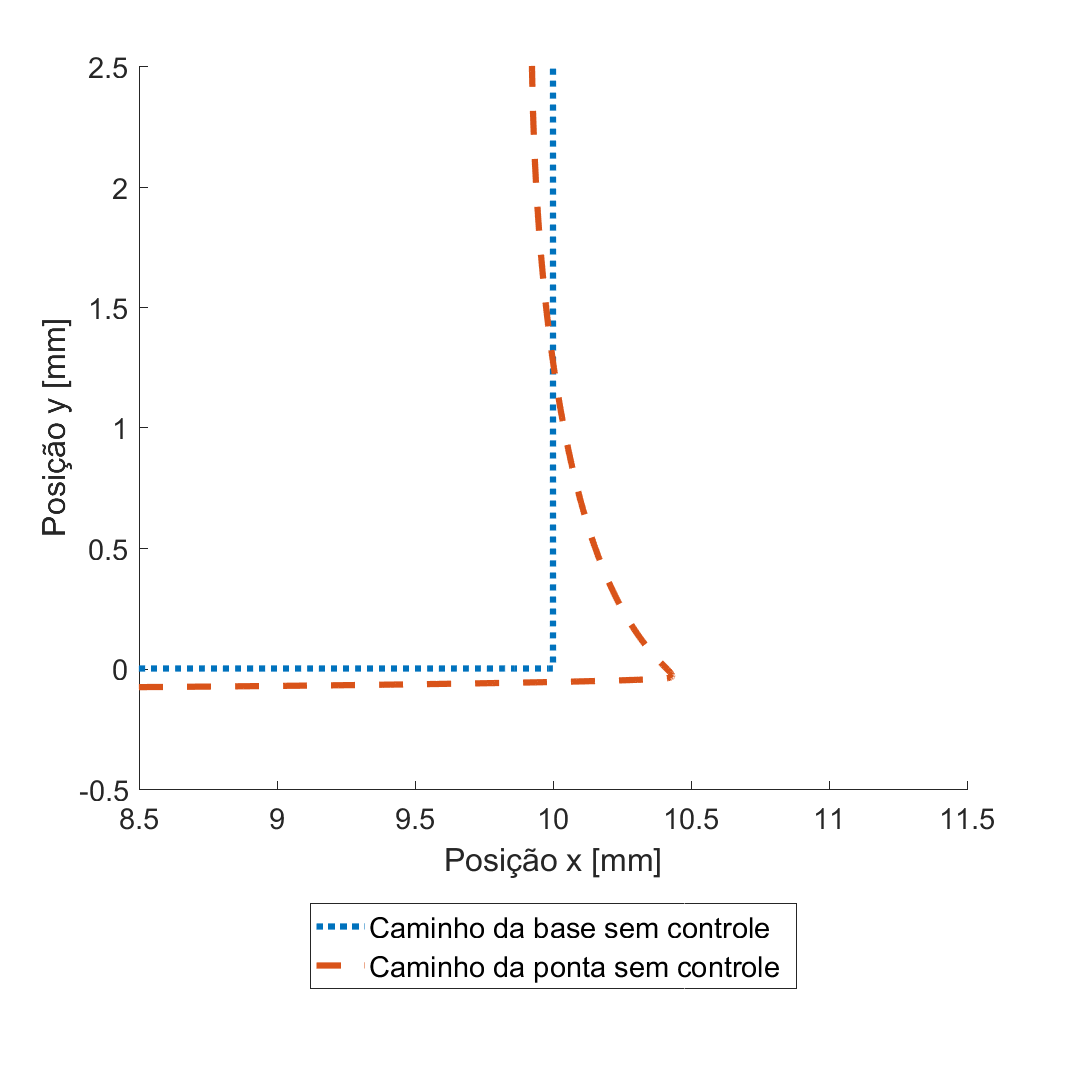
\includegraphics[width=0.47\textwidth]{Sim ref_cam_s_zoom.png}
        \label{fig:ref_cam_s_zoom}
    }
    \hfill
    \subfigure[Detalhamento - Com controle.]{
        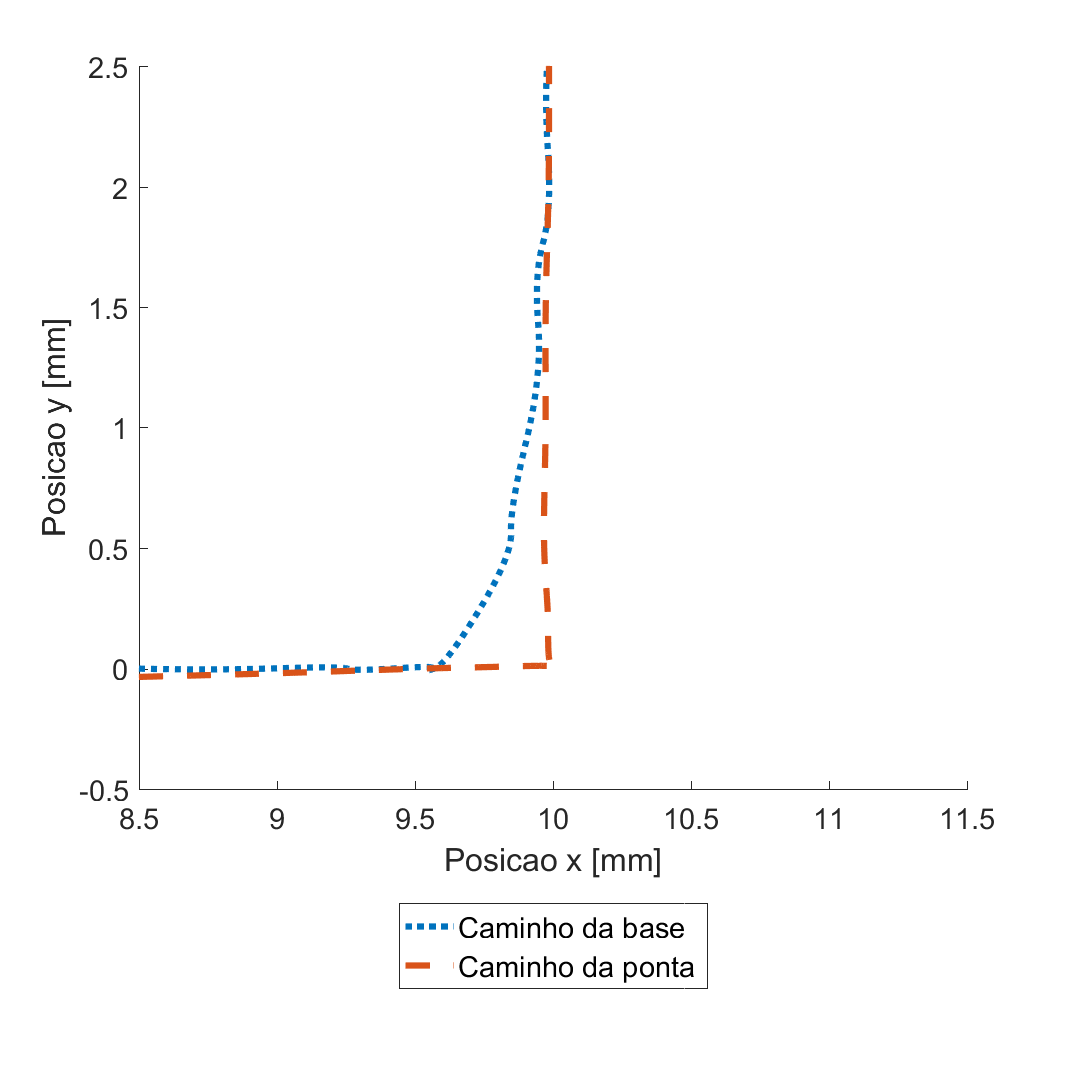
\includegraphics[width=0.47\textwidth]{Sim ref_cam_c_zoom.png}
        \label{fig:ref_cam_c_zoom}
    }
    \caption{Caminhos da ponta e da base - Referência.}
    \label{fig:ref_cam}
\end{figure}

A partir deste gráfico, é possível identificar que o comportamento do arredondamento da curva do caminho da base está relacionado à compensação do sobre-sinal resultante do comportamento dinâmico da impressora, visível no caminho da ponta sem o controle de trajetória, ou seja, a trajetória da base é igual à trajetória de entrada na etapa do controle de trajetória.

% ------------------ Deslocamento ----------------
Já na Figura \ref{fig:ref_des} é visível alguns comportamentos dinâmicos das curvas de deslocamento. No início do movimento, a curva da base se desloca mais rapidamente, também sendo possível observar algumas oscilações. Enquanto a curva da ponta sem controle apresenta um deslocamento mais lento, característica essa evitada pelo controle de trajetória, resultando em uma curva mais suave para o deslocamento com controle.

% fig:des
\begin{figure}[H]
    \centering
    \subfigure[Sem controle.]{
        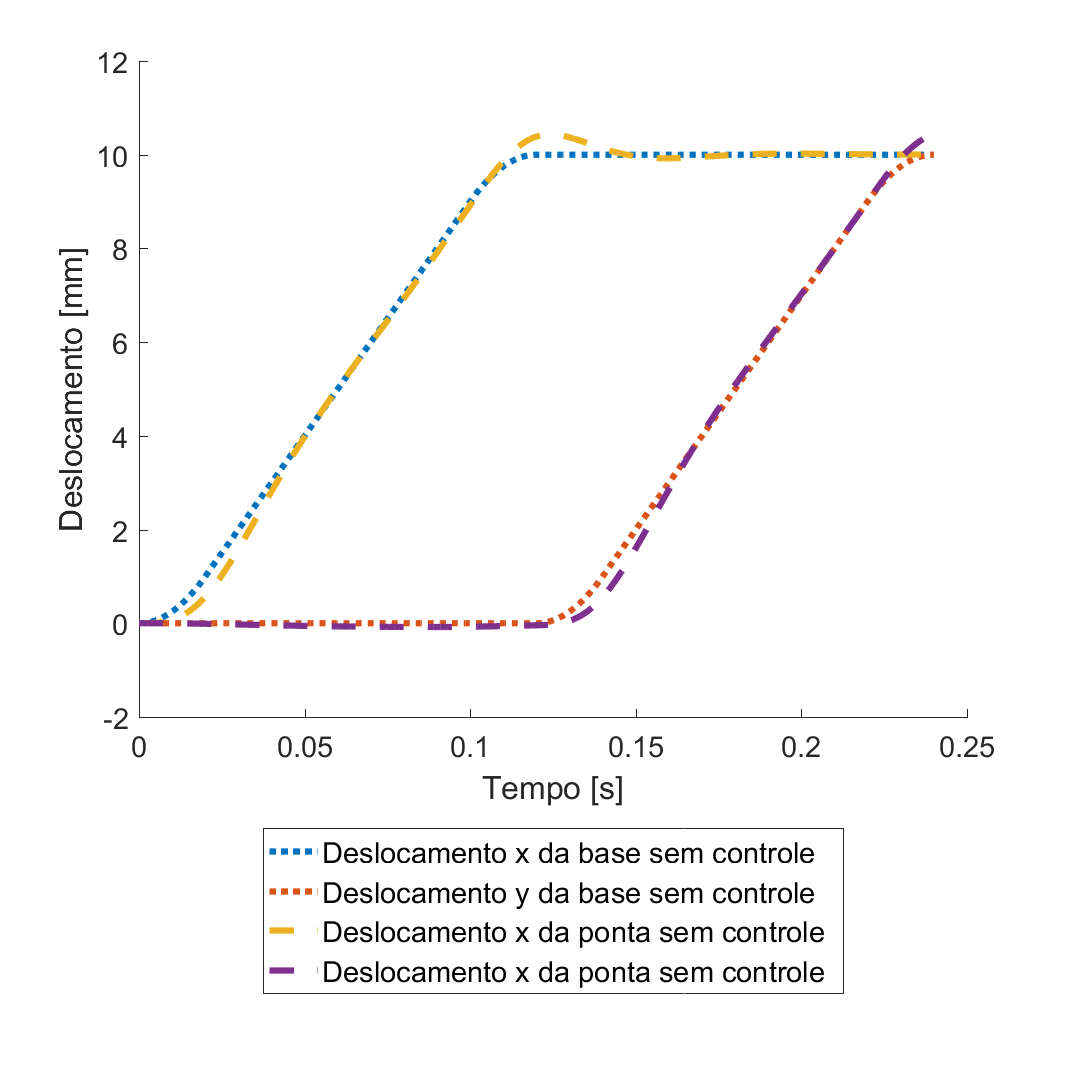
\includegraphics[width=0.47\textwidth]{Sim ref_des_s.png}
        \label{fig:ref_des_s}
    }
    \hfill
    \subfigure[Com controle.]{
        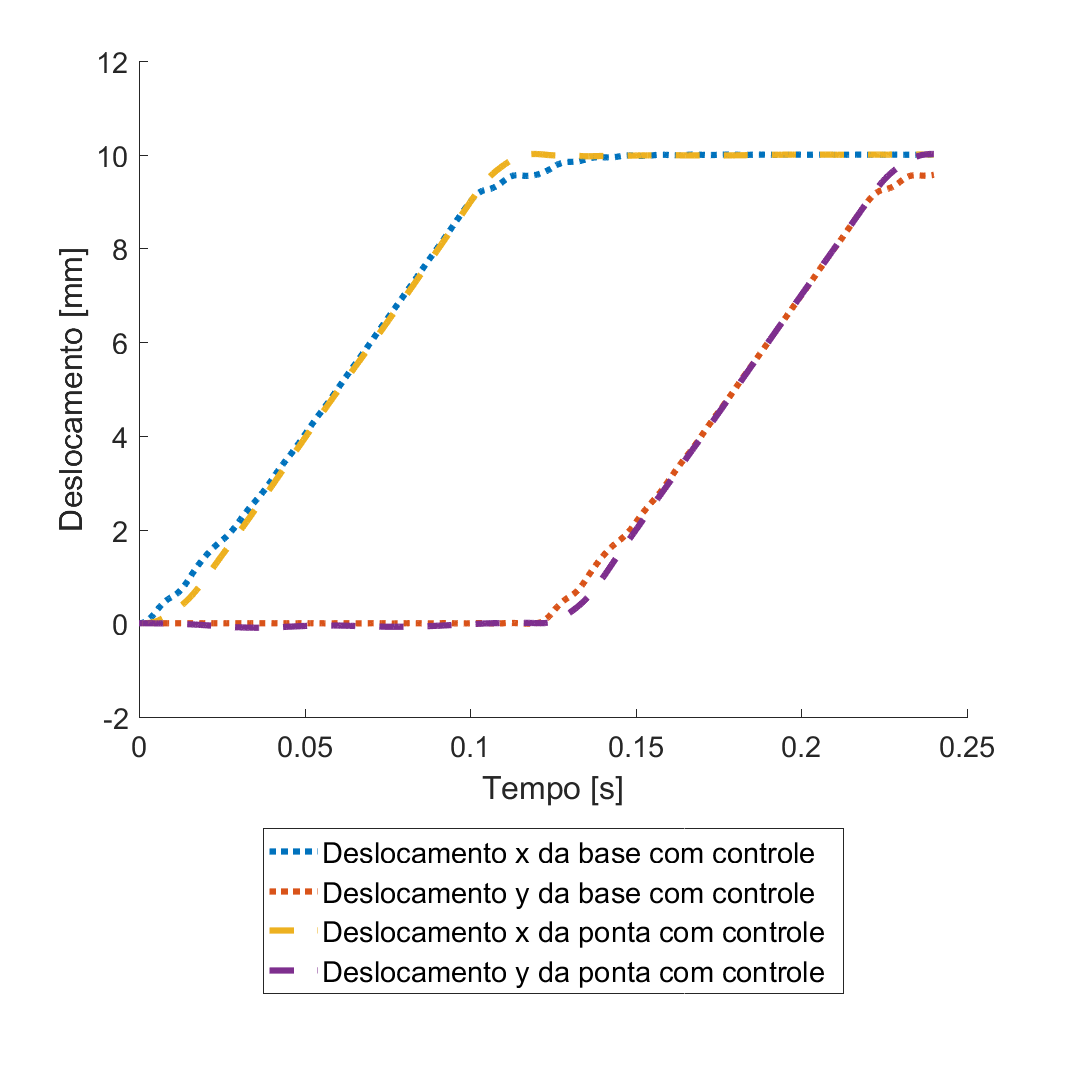
\includegraphics[width=0.47\textwidth]{Sim ref_des_c.png}
        \label{fig:ref_des_c}
    }
    \caption{Deslocamentos da ponta e da base - Referência.}
    \label{fig:ref_des}
\end{figure}

Além disso, no fim do movimento em X podemos observar um sobre-sinal considerável na curva de deslocamento da ponta sem controle. Em contrapartida, a curva de deslocamento da base conseguiu compensar consideravelmente a característica elástica do sistema, apresentando um sobre-sinal muito menor na curva de deslocamento da ponta com controle.

% ------------------ Velocidades ----------------
Outra característica notável neste gráfico (Figura \ref{fig:ref_vel_b}) é a oscilação aguda, dado o passo de tempo relativamente grande considerando a frequência das oscilações. Esse efeito é minimizado na Figura \ref{fig:ref_vel_p} por causa da interpolação necessária para se aplicar o método Runge-Kutta com sucesso, como discutido anteriormente, além disso a própria dinâmica da impressora pode amenizar essas oscilações, sendo este efeito uma combinação de fatores.

% fig:vel
\begin{figure}[H]
    \centering
    \subfigure[Sem controle.]{
        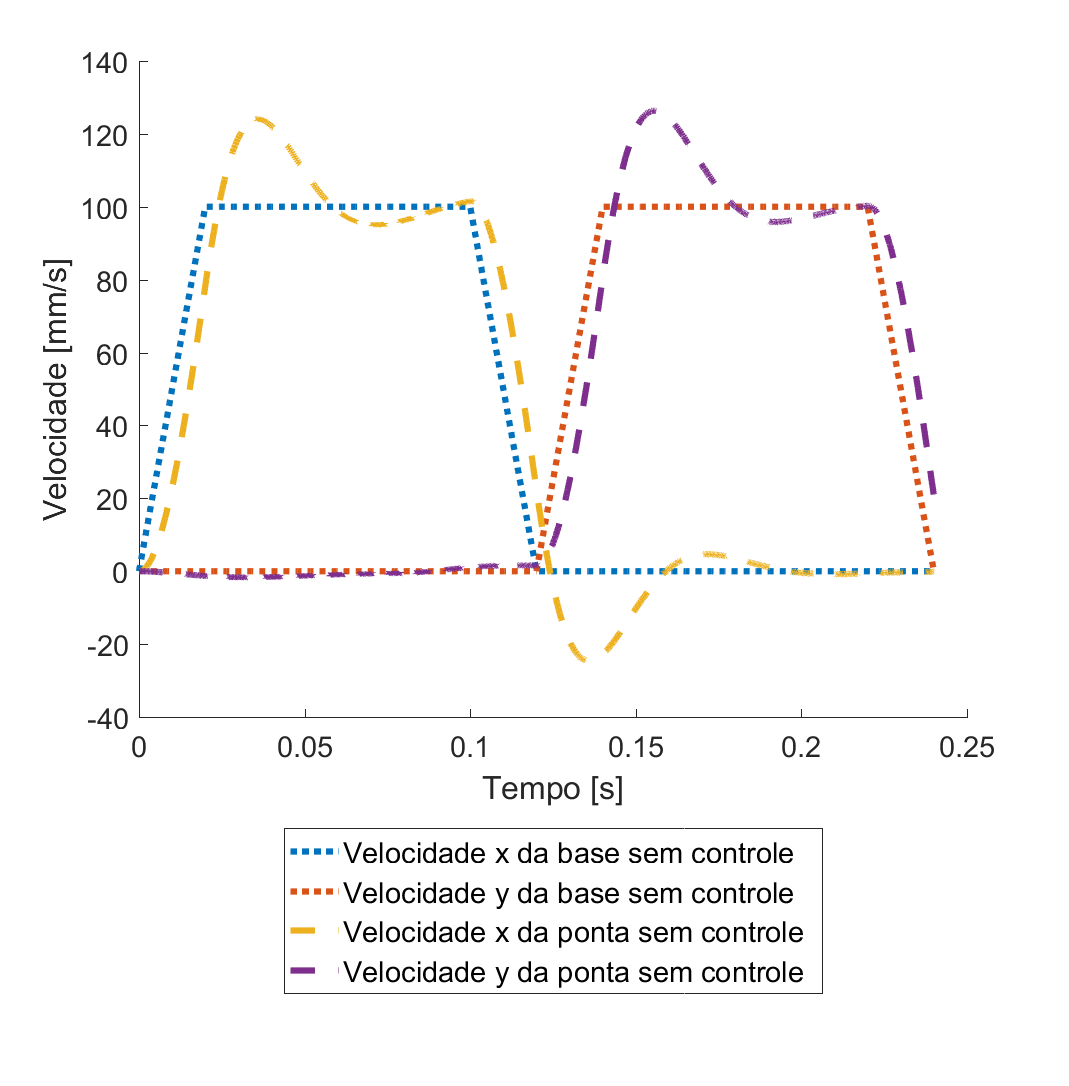
\includegraphics[width=0.47\textwidth]{Sim ref_vel_s.png}
        \label{fig:ref_vel_s}
    }
    \hfill
    \subfigure[Com controle.]{
        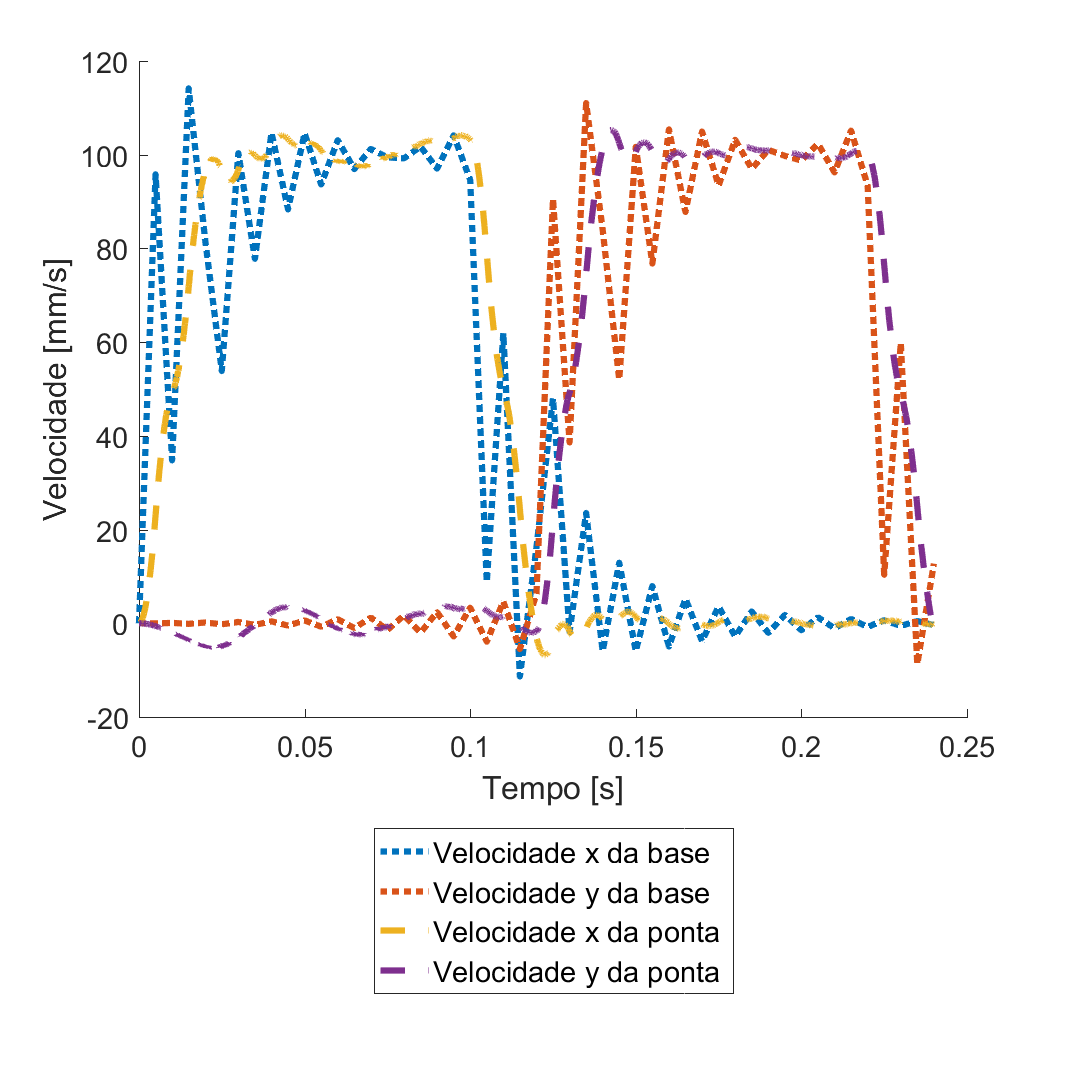
\includegraphics[width=0.47\textwidth]{Sim ref_vel_c.png}
        \label{fig:ref_vel_c}
    }
    \caption{Velocidades da ponta e da base - Referência.}
    \label{fig:ref_vel}
\end{figure}

Observa-se também na Figura \ref{fig:ref_vel_p} que a curva de velocidade da ponta com controle se aproxima mais fielmente à trajetória de entrada do controle de trajetória, enquanto a curva de velocidade sem controle apresenta sobre-sinais mais acentuados, que corrobora com as características das curvas de deslocamento e de caminho discutidas anteriormente.
A análise das velocidades X e Y da base, conforme mostrado no quinto gráfico, revela um perfil de velocidade que varia de acordo com as exigências da trajetória. A resposta do sistema em ambas as direções permanece dentro de um envelope controlado, indicativo de um comportamento robusto do sistema de controle frente às demandas dinâmicas do movimento.
% ------------------ end ----------------

\subsection{Caso 1 - Variação da frequência natural}
A partir desta seção são avaliados os resultados das simulações com a variação dos parâmetros, com seus valores inferiores (A) e superiores (B), comparando com os resultados da simulação referência, estes apresentados na seção anterior.

% ------------------ Caminho A ----------------

Neste primeiro gráfico (Figura \ref{fig:1A_cam_b}) é apresentado o caminho da base da simulação com o parâmetro da frequência natural em seu nível inferior, definido como \(50 rad/s\). Nota-se algumas características em comum com a Figura \ref{fig:ref_cam_b} da simulação referência, mas peculiarmente é possível observar um ponto onde o caminho da base se sobrepõe no eixo X.

% fig:cam
\begin{figure}[H]
    \centering
    \subfigure[Sem controle.]{
        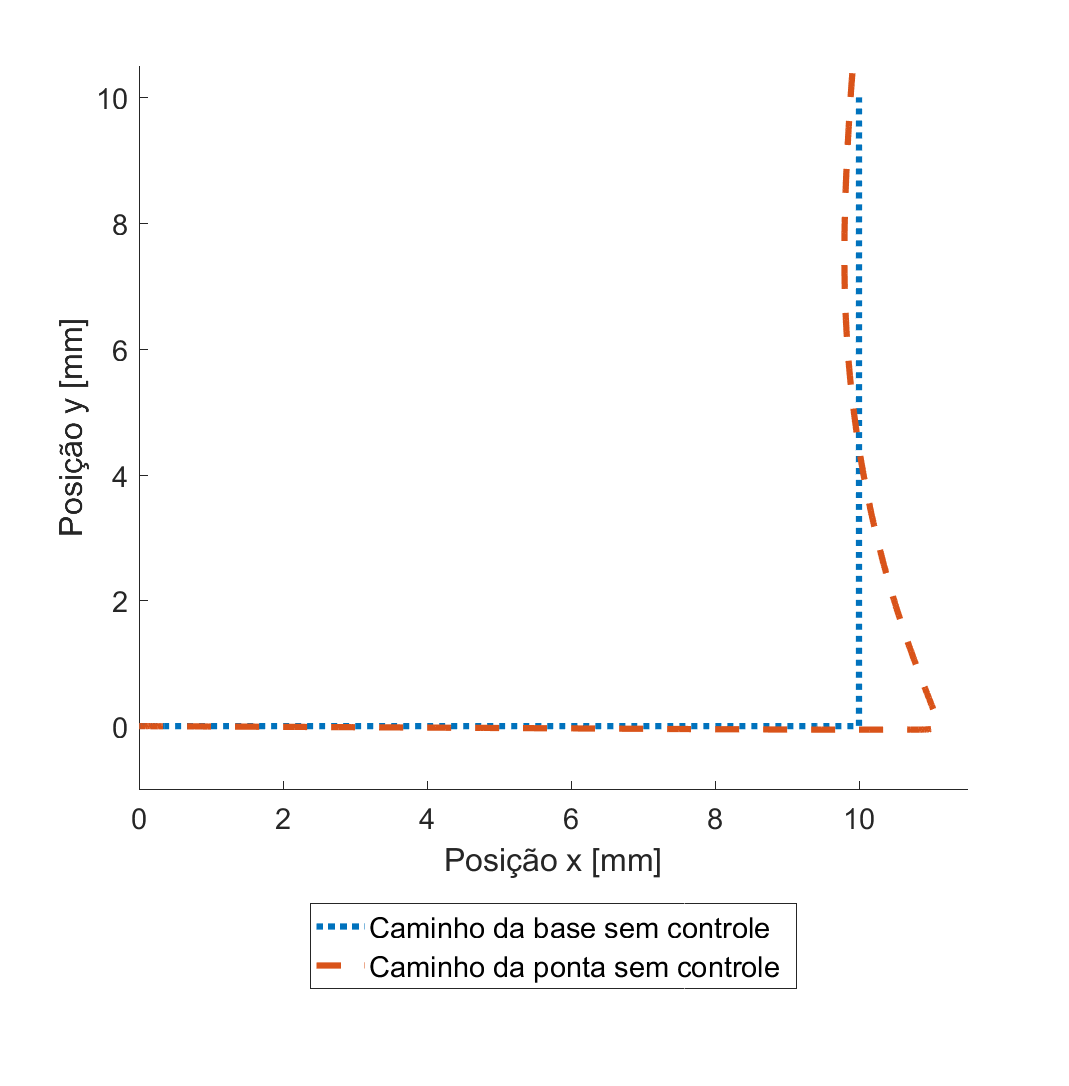
\includegraphics[width=0.47\textwidth]{Sim 1A_cam_s.png}
        \label{fig:1A_cam_s}
    }
    \hfill
    \subfigure[Com controle.]{
        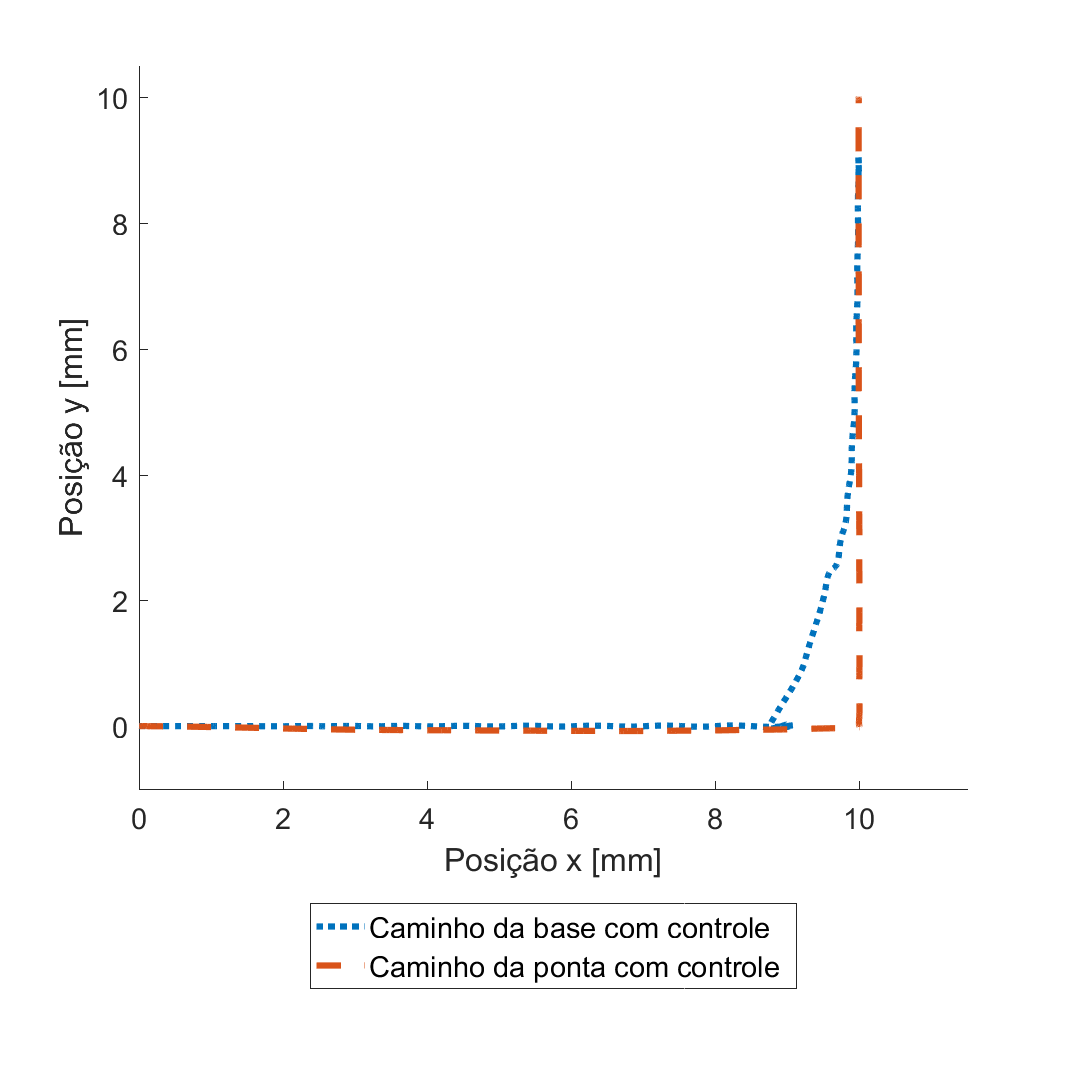
\includegraphics[width=0.47\textwidth]{Sim 1A_cam_c.png}
        \label{fig:1A_cam_c}
    }
    \hfill
    \subfigure[Detalhamento - Sem controle.]{
        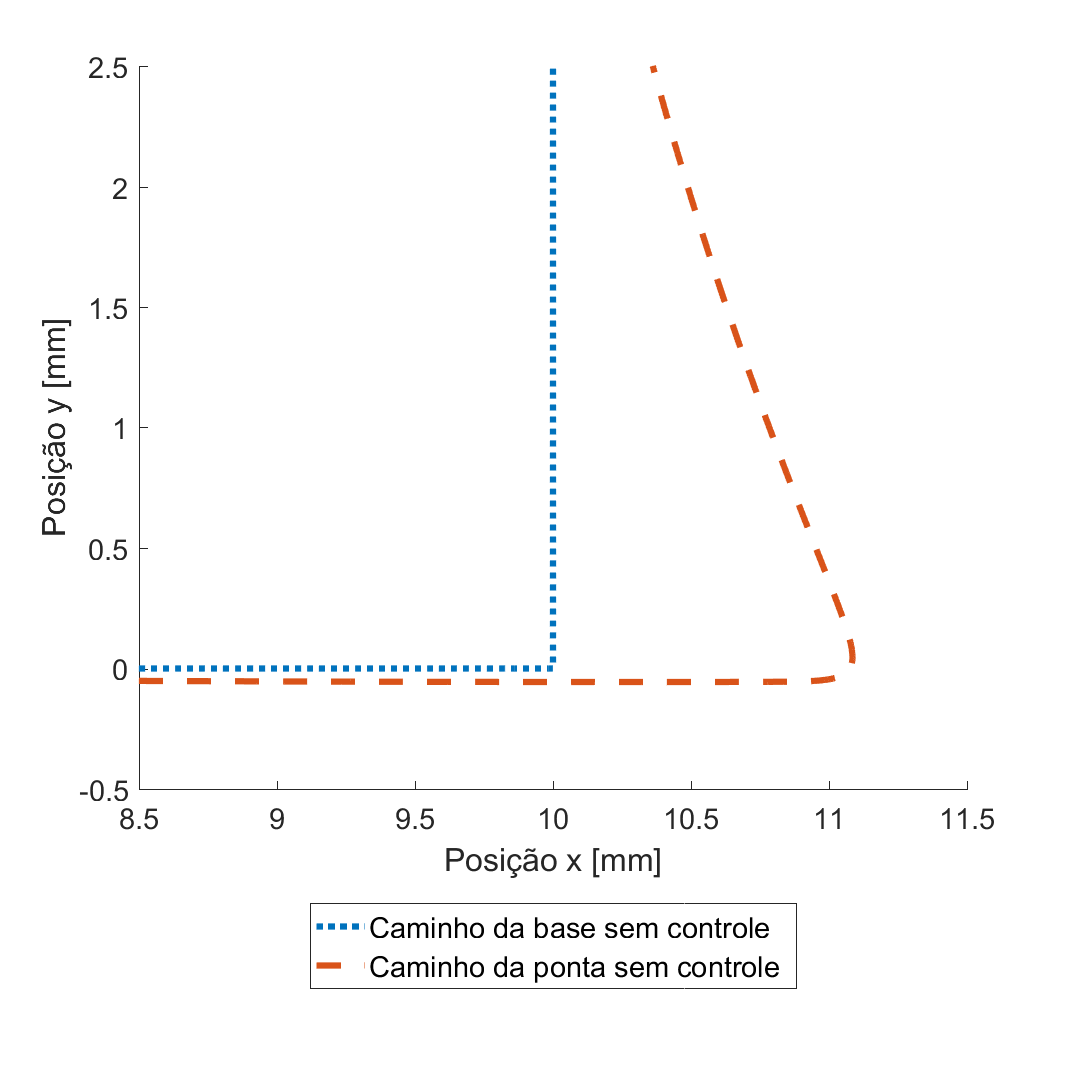
\includegraphics[width=0.47\textwidth]{Sim 1A_cam_s_zoom.png}
        \label{fig:1A_cam_s_zoom}
    }
    \hfill
    \subfigure[Detalhamento - Com controle.]{
        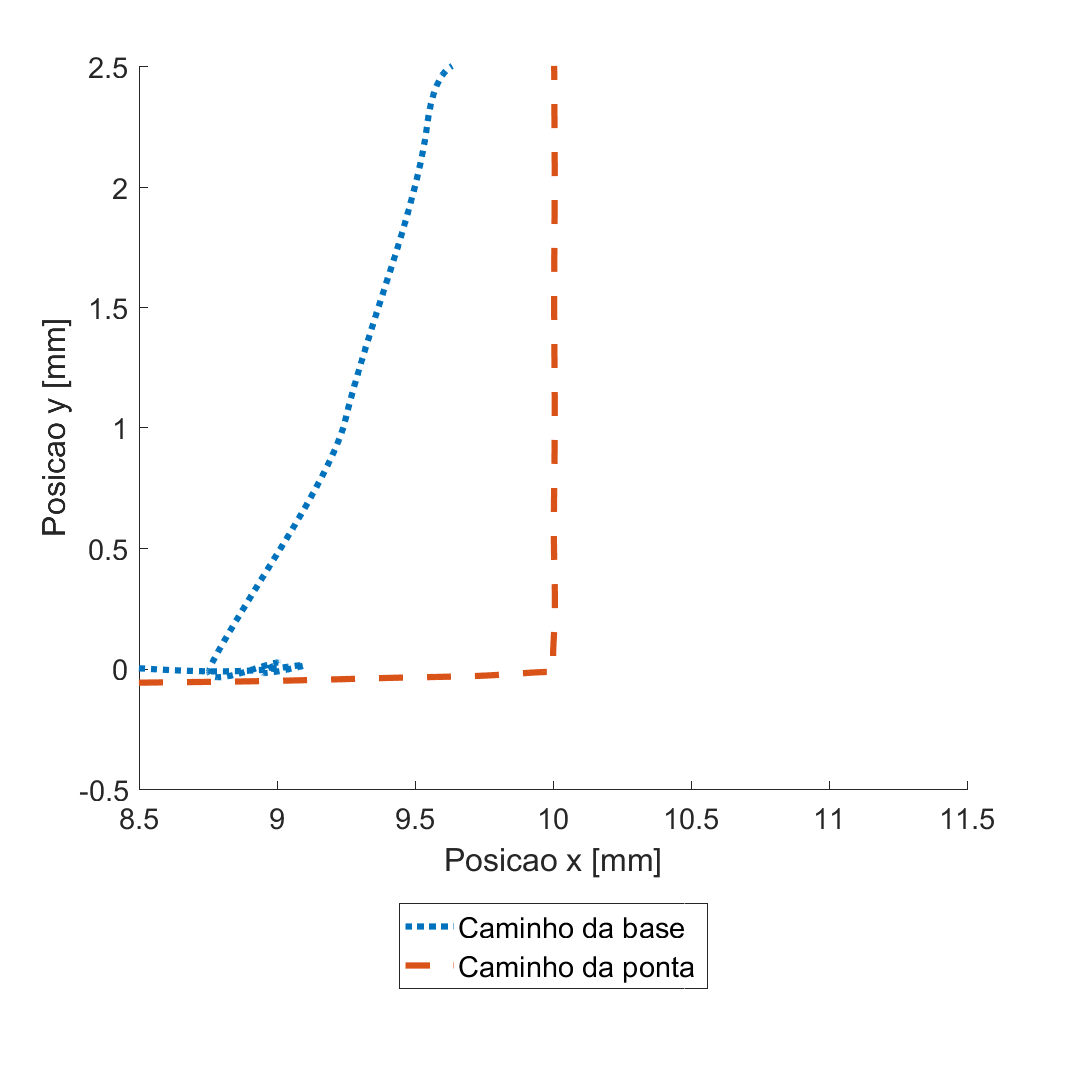
\includegraphics[width=0.47\textwidth]{Sim 1A_cam_c_zoom.png}
        \label{fig:1A_cam_c_zoom}
    }
    \caption{Caminhos da ponta e da base - Caso 1A.}
    \label{fig:1A_cam}
\end{figure}

Este comportamento é justificado quando se analisa a Figura \ref{fig:1A_cam_p_s}, que exibe um sobre-sinal mais forte do que antes visto na simulação de referência, necessitando uma compensação maior para se atenuar este efeito. Entretanto, o caminho da ponta com controle ainda se mantém próximo ao caminho desejado, demonstrando êxito na atenuação do sobre-sinal e da oscilação em sua sequência.

% ------------------ Caminho B ----------------

Fisicamente este resultado está condizente com a redução da frequência natural, que caracteriza em um aumento da elasticidade e por consequência no aumento da amplitude nessas condições. Na Figura \ref{fig:1B_cam_p_s} também podemos observar o resultado da simulação do valor superior da frequência natural, \(200 rad/s\). 

% fig:cam
\begin{figure}[H]
    \centering
    \subfigure[Sem controle.]{
        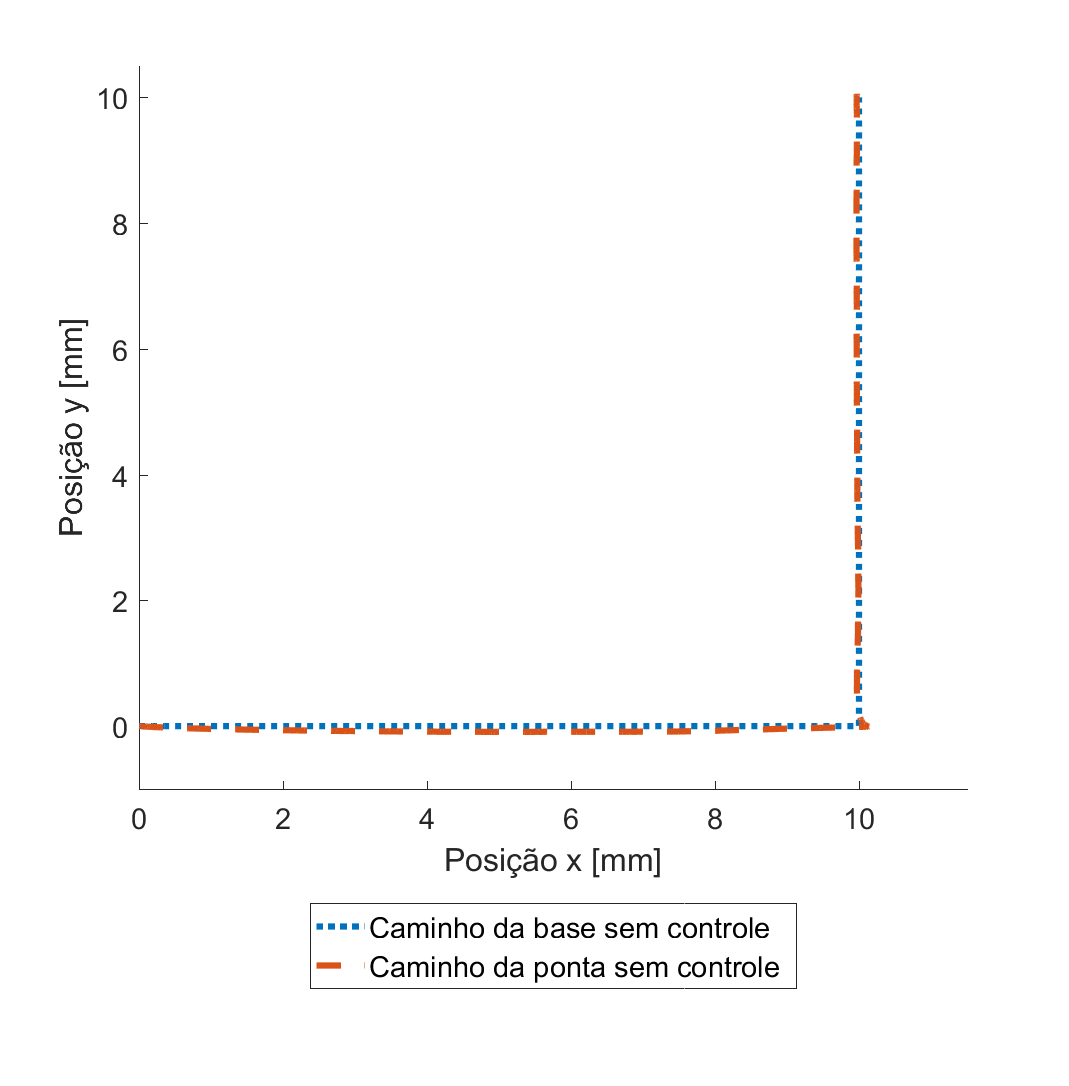
\includegraphics[width=0.47\textwidth]{Sim 1B_cam_s.png}
        \label{fig:1B_cam_s}
    }
    \hfill
    \subfigure[Com controle.]{
        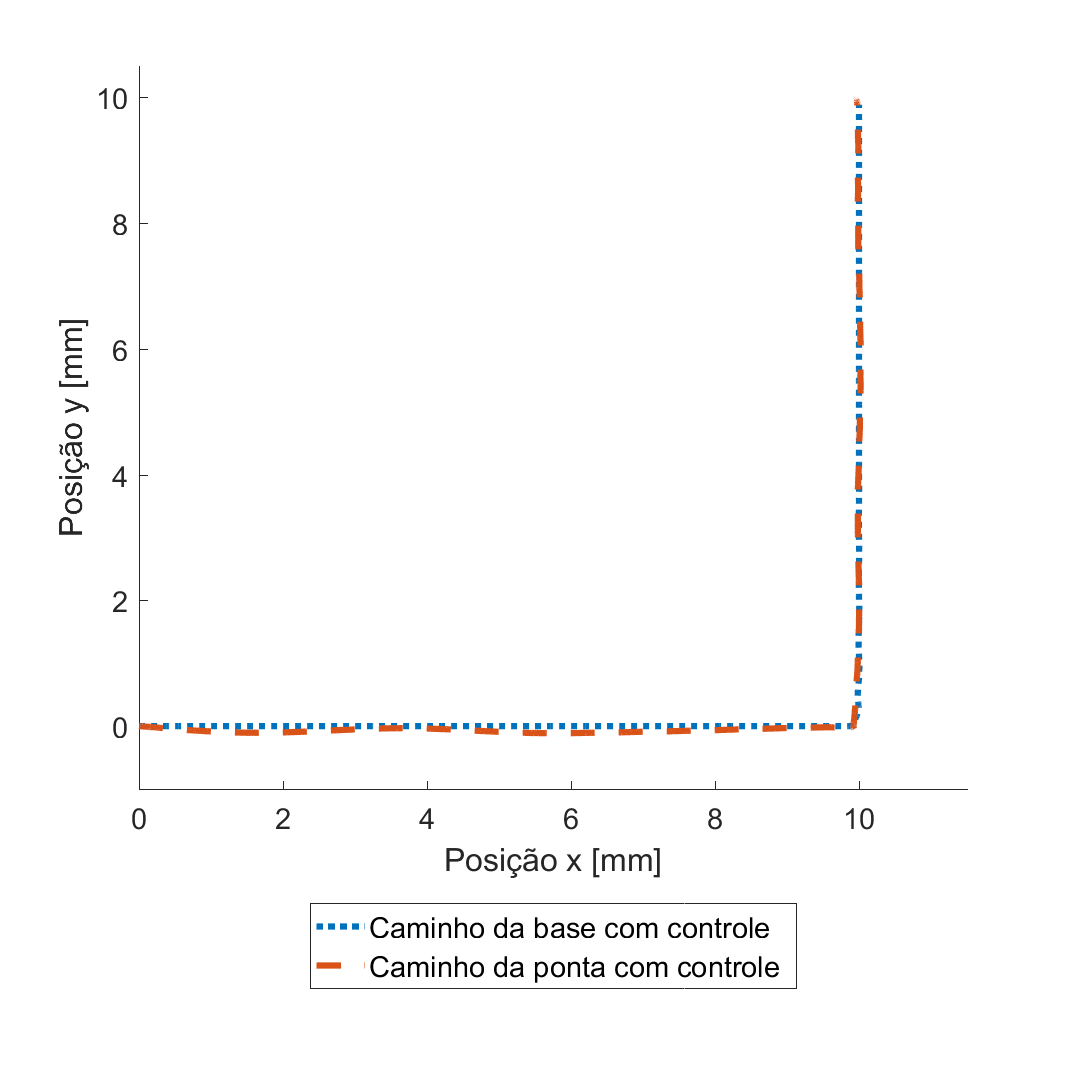
\includegraphics[width=0.47\textwidth]{Sim 1B_cam_c.png}
        \label{fig:1B_cam_c}
    }
    \hfill
    \subfigure[Detalhamento - Sem controle.]{
        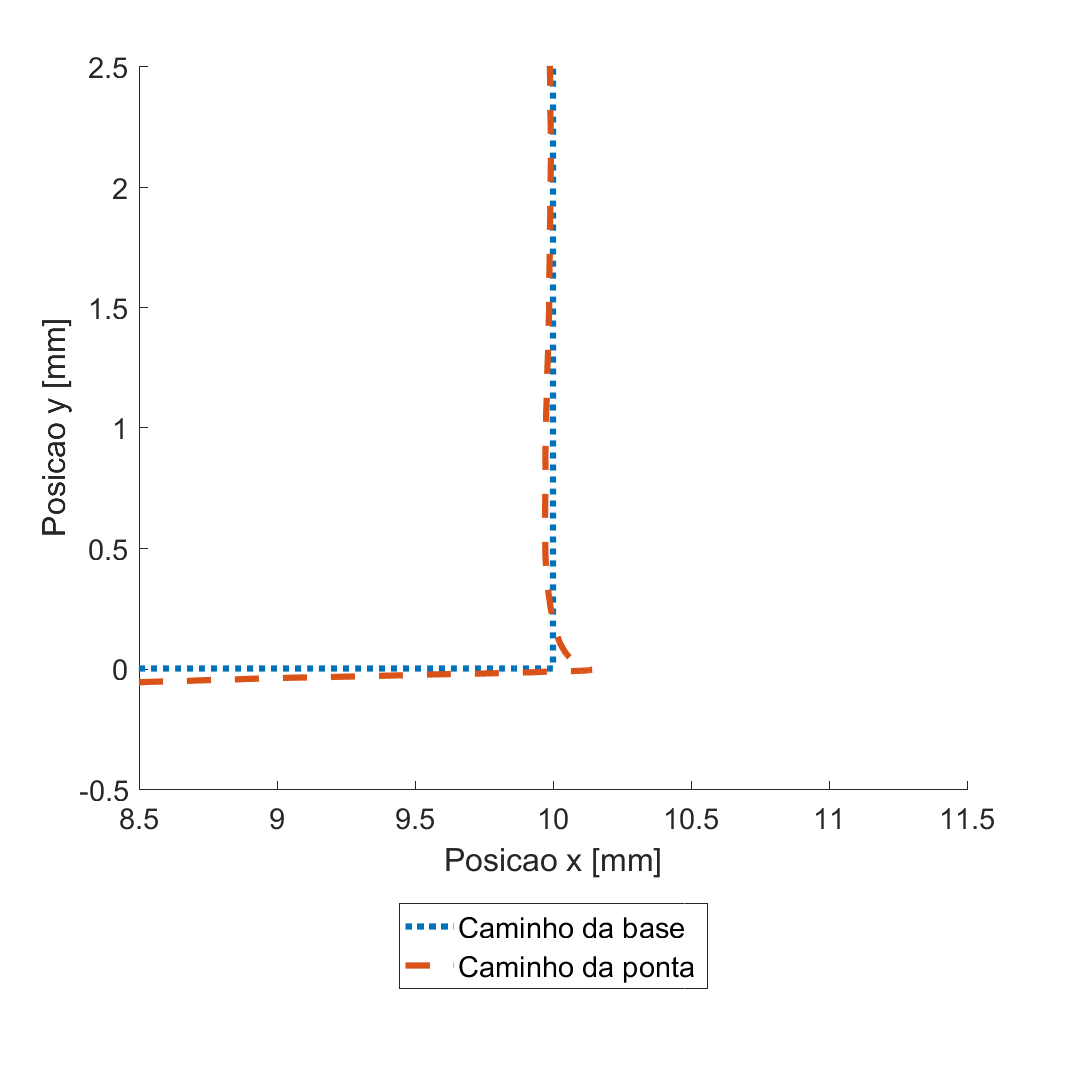
\includegraphics[width=0.47\textwidth]{Sim 1B_cam_s_zoom.png}
        \label{fig:1B_cam_s_zoom}
    }
    \hfill
    \subfigure[Detalhamento - Com controle.]{
        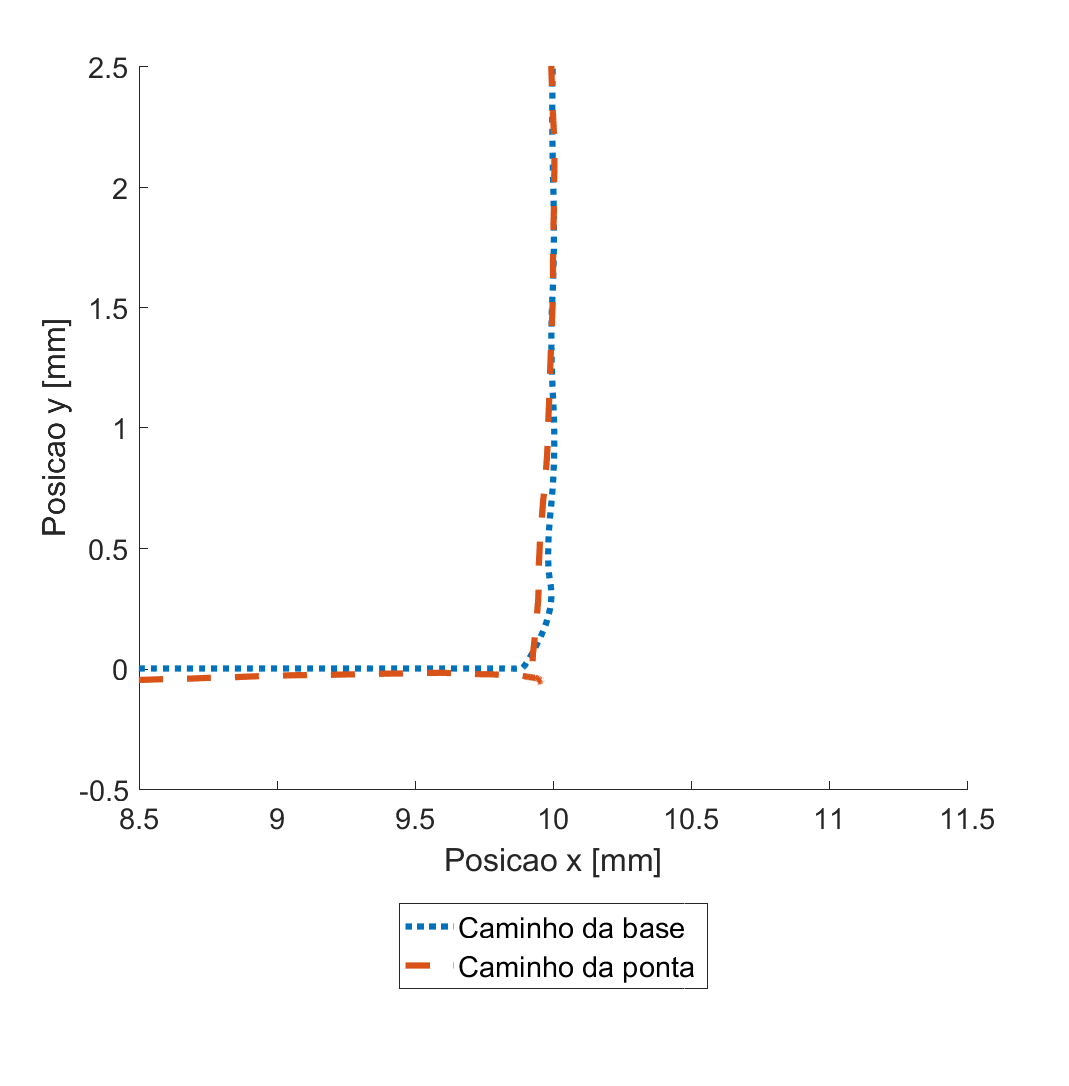
\includegraphics[width=0.47\textwidth]{Sim 1B_cam_c_zoom.png}
        \label{fig:1B_cam_c_zoom}
    }
    \caption{Caminhos da ponta e da base - Caso 1B.}
    \label{fig:1B_cam}
\end{figure}

Nota-se que com o aumento da frequência natural existe uma amenização no sobre-sinal e nas amplitudes das oscilações nessas condições. Esta característica corrobora com os resultados anteriores, agora promovendo uma rigidez no sistema e diminuindo a discrepância entre os caminhos da ponta com controle e sem controle. Entretanto, a precisão do caminho da ponta com controle foi afetada, dada essas condições.

% ------------------ Deslocamento A----------------

% fig:des
\begin{figure}[H]
    \centering
    \subfigure[Sem controle.]{
        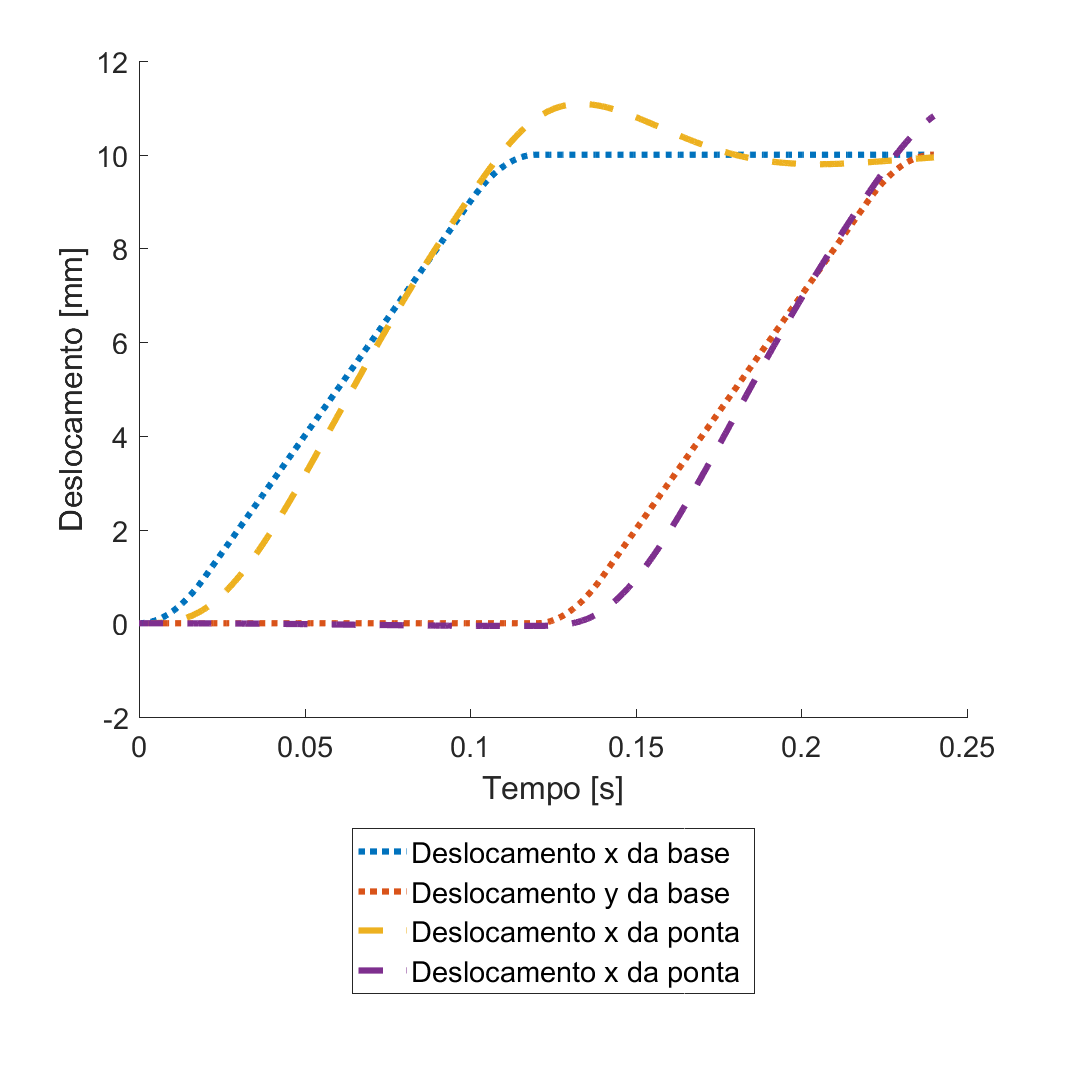
\includegraphics[width=0.47\textwidth]{Sim 1A_des_s.png}
        \label{fig:1A_des_s}
    }
    \hfill
    \subfigure[Com controle.]{
        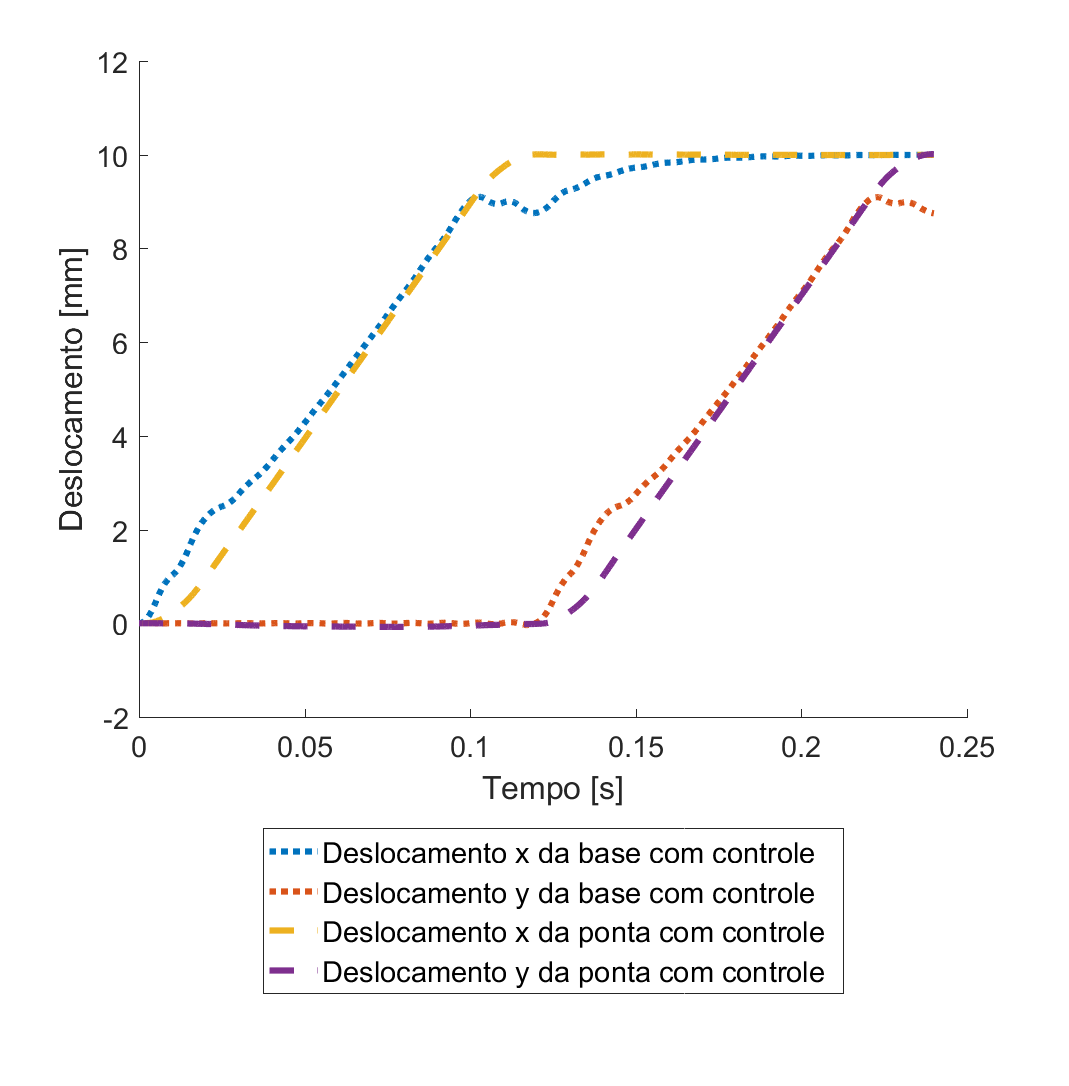
\includegraphics[width=0.47\textwidth]{Sim 1A_des_c.png}
        \label{fig:1A_des_c}
    }
    \caption{Deslocamentos da ponta e da base - Caso 1A.}
    \label{fig:1A_des}
\end{figure}

% ------------------ Deslocamento B----------------

% fig:des
\begin{figure}[H]
    \centering
    \subfigure[Sem controle.]{
        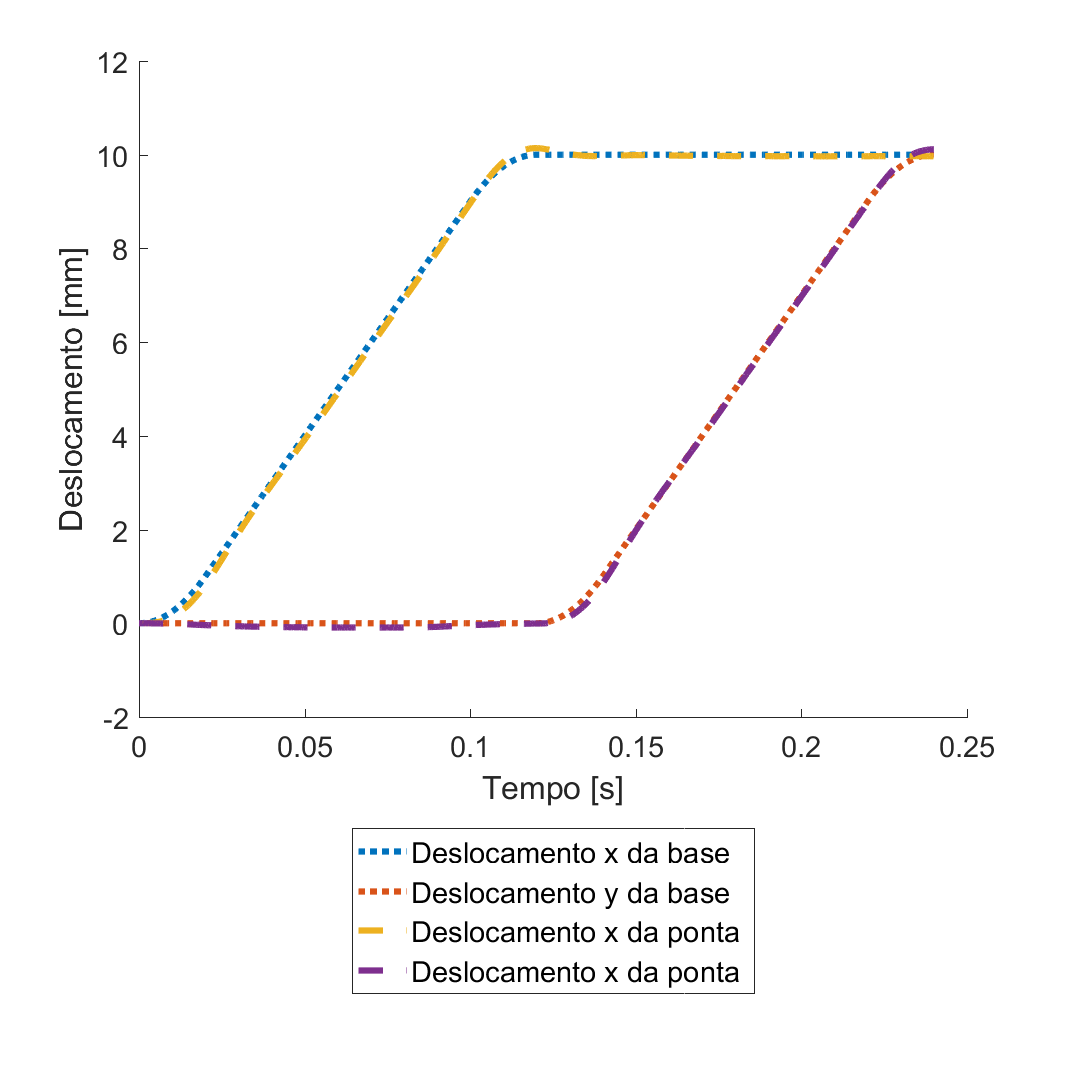
\includegraphics[width=0.47\textwidth]{Sim 1B_des_s.png}
        \label{fig:1B_des_s}
    }
    \hfill
    \subfigure[Com controle.]{
        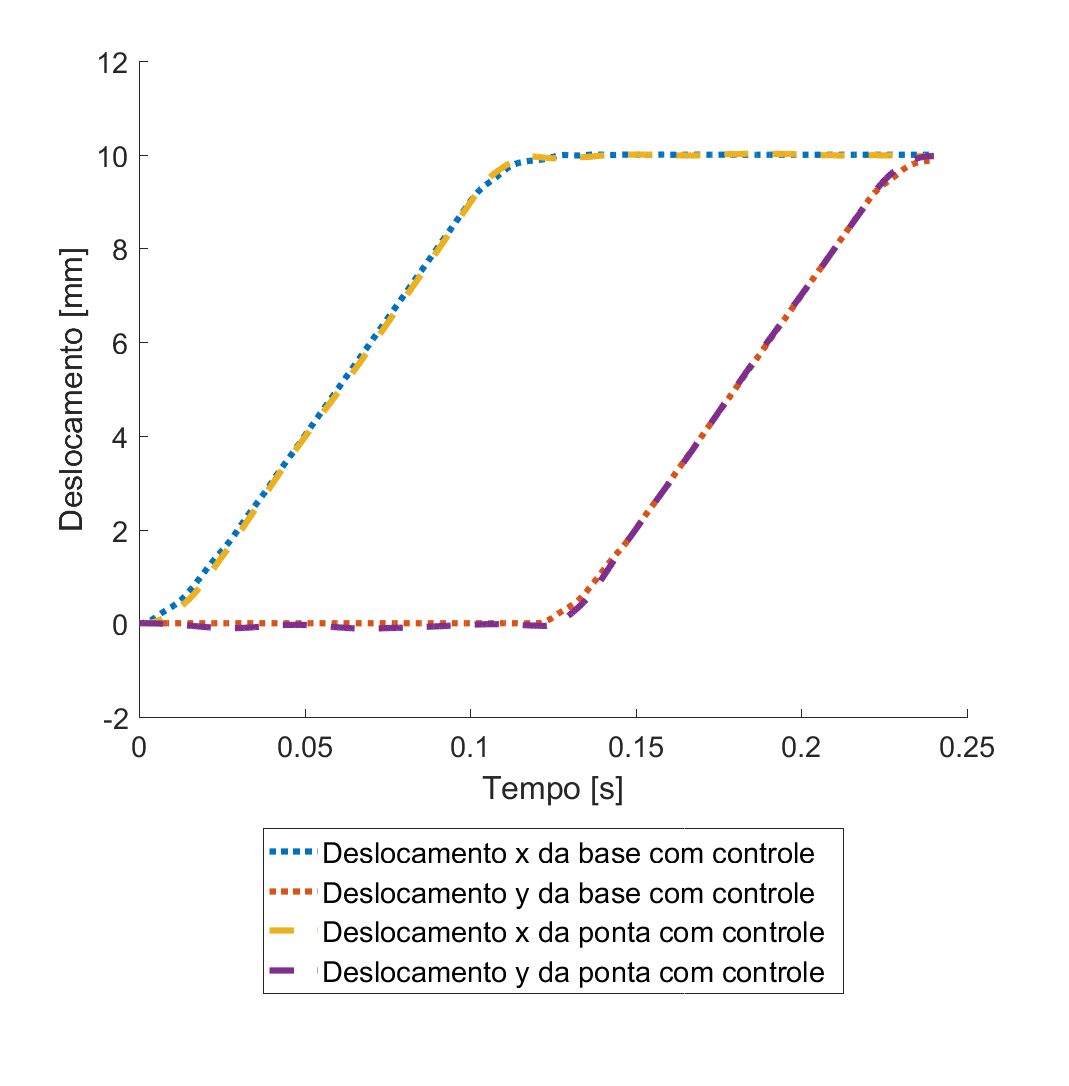
\includegraphics[width=0.47\textwidth]{Sim 1B_des_c.png}
        \label{fig:1B_des_c}
    }
    \caption{Deslocamentos da ponta e da base - Caso 1B.}
    \label{fig:1B_des}
\end{figure}

% ------------------ Velocidades A ----------------

% fig:vel
\begin{figure}[H]
    \centering
    \subfigure[Sem controle.]{
        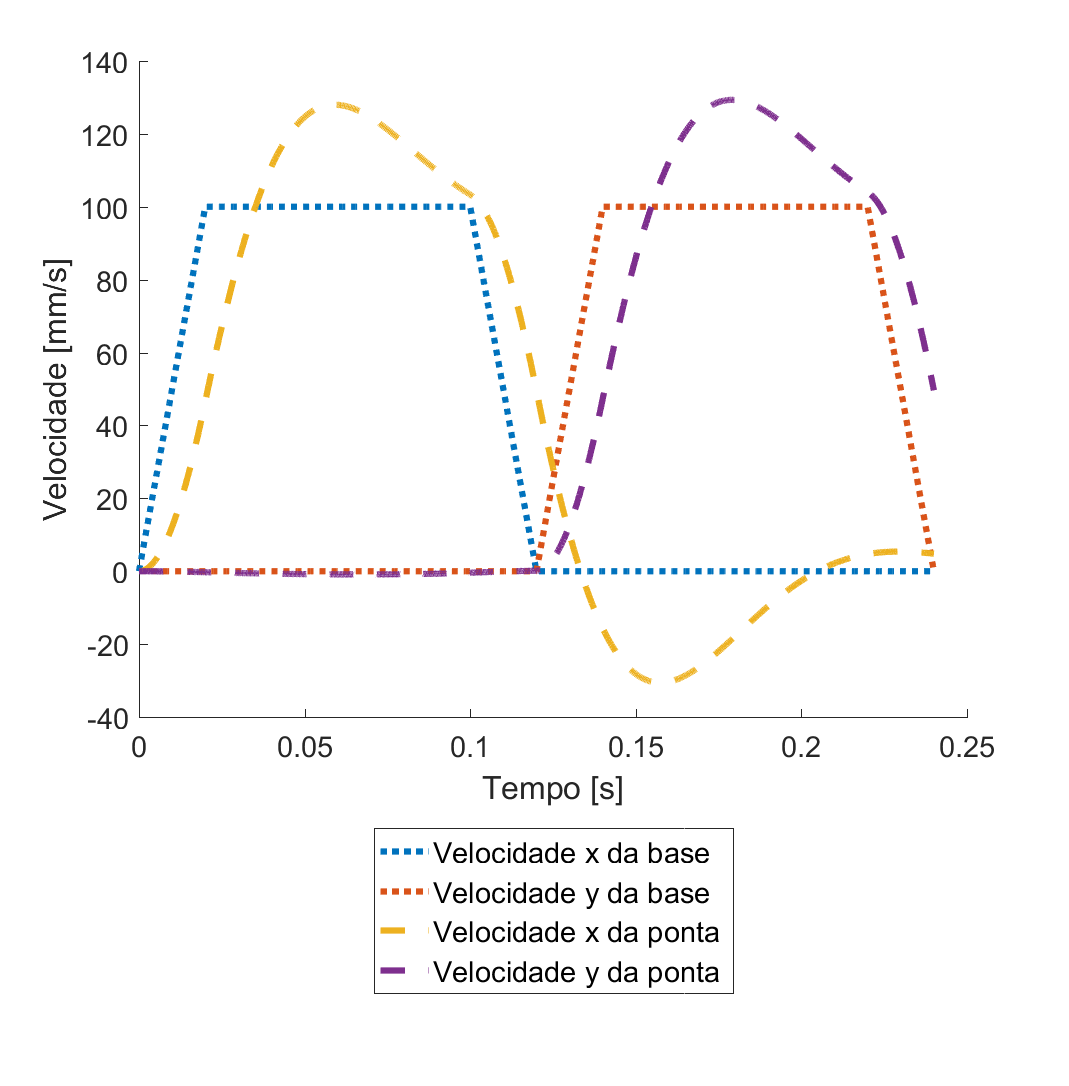
\includegraphics[width=0.47\textwidth]{Sim 1A_vel_s.png}
        \label{fig:1A_vel_s}
    }
    \hfill
    \subfigure[Com controle.]{
        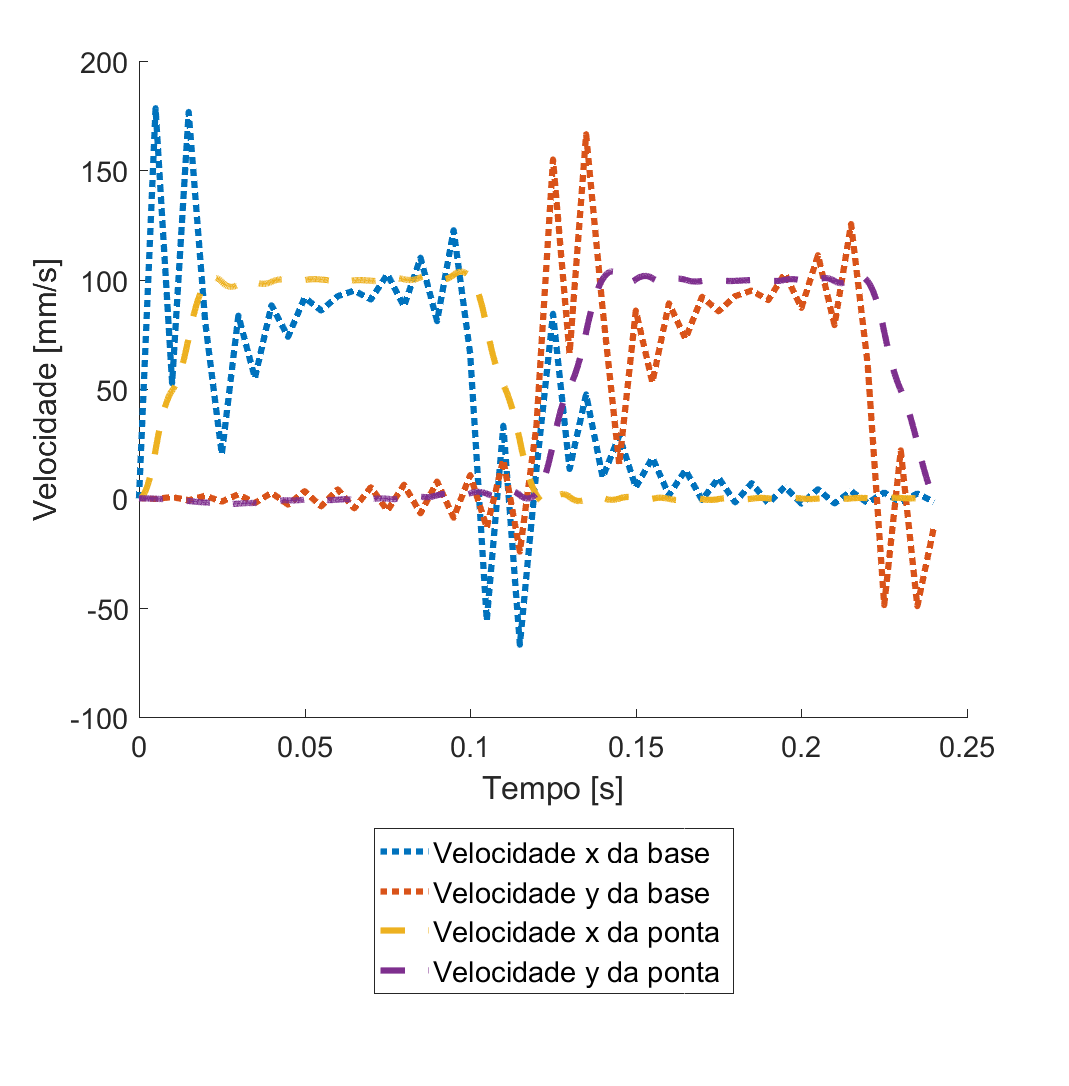
\includegraphics[width=0.47\textwidth]{Sim 1A_vel_c.png}
        \label{fig:1A_vel_c}
    }
    \caption{Velocidades da ponta e da base - Caso 1A.}
    \label{fig:1A_vel}
\end{figure}

% ------------------ Velocidades B ----------------

% fig:vel
\begin{figure}[H]
    \centering
    \subfigure[Sem controle.]{
        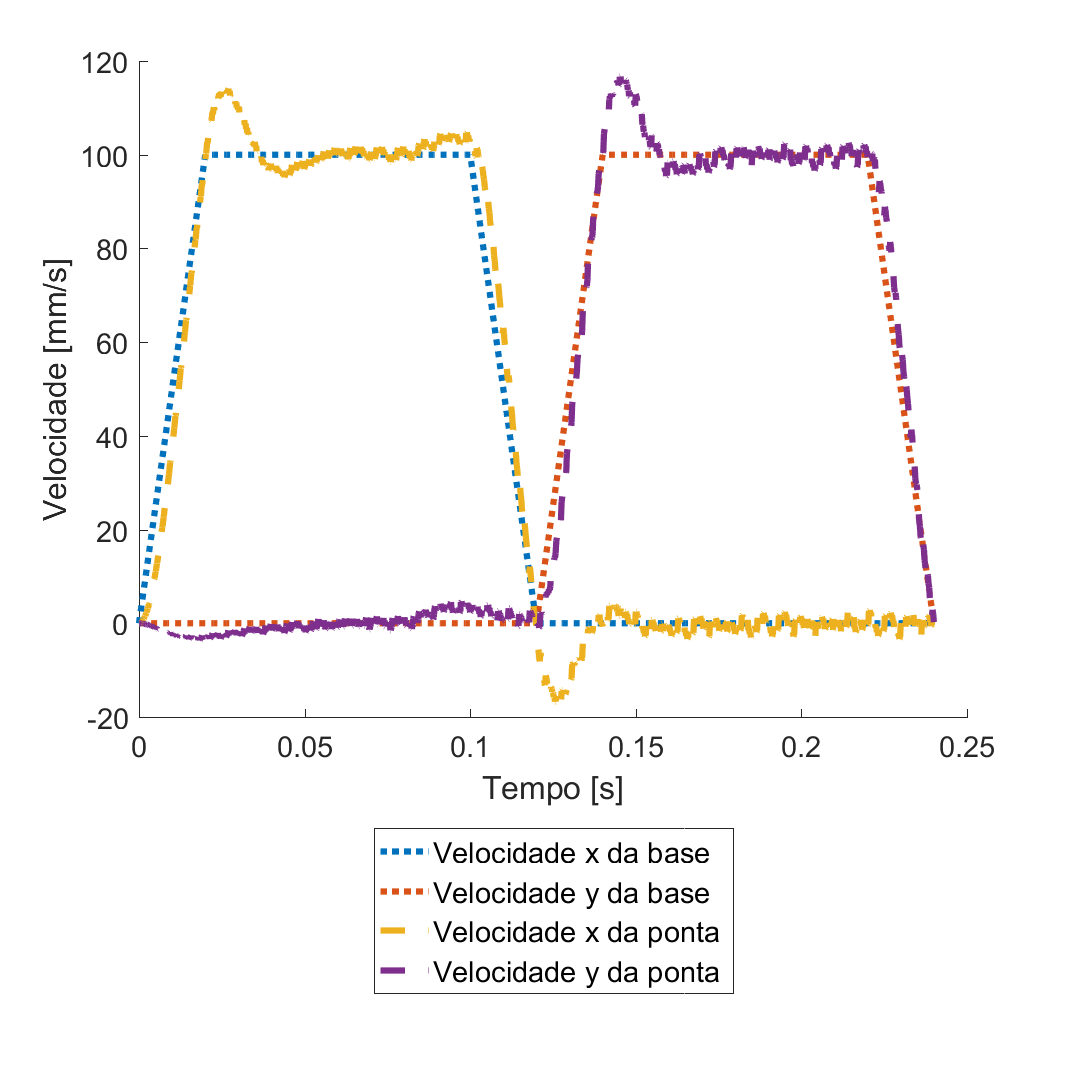
\includegraphics[width=0.47\textwidth]{Sim 1B_vel_s.png}
        \label{fig:1B_vel_s}
    }
    \hfill
    \subfigure[Com controle.]{
        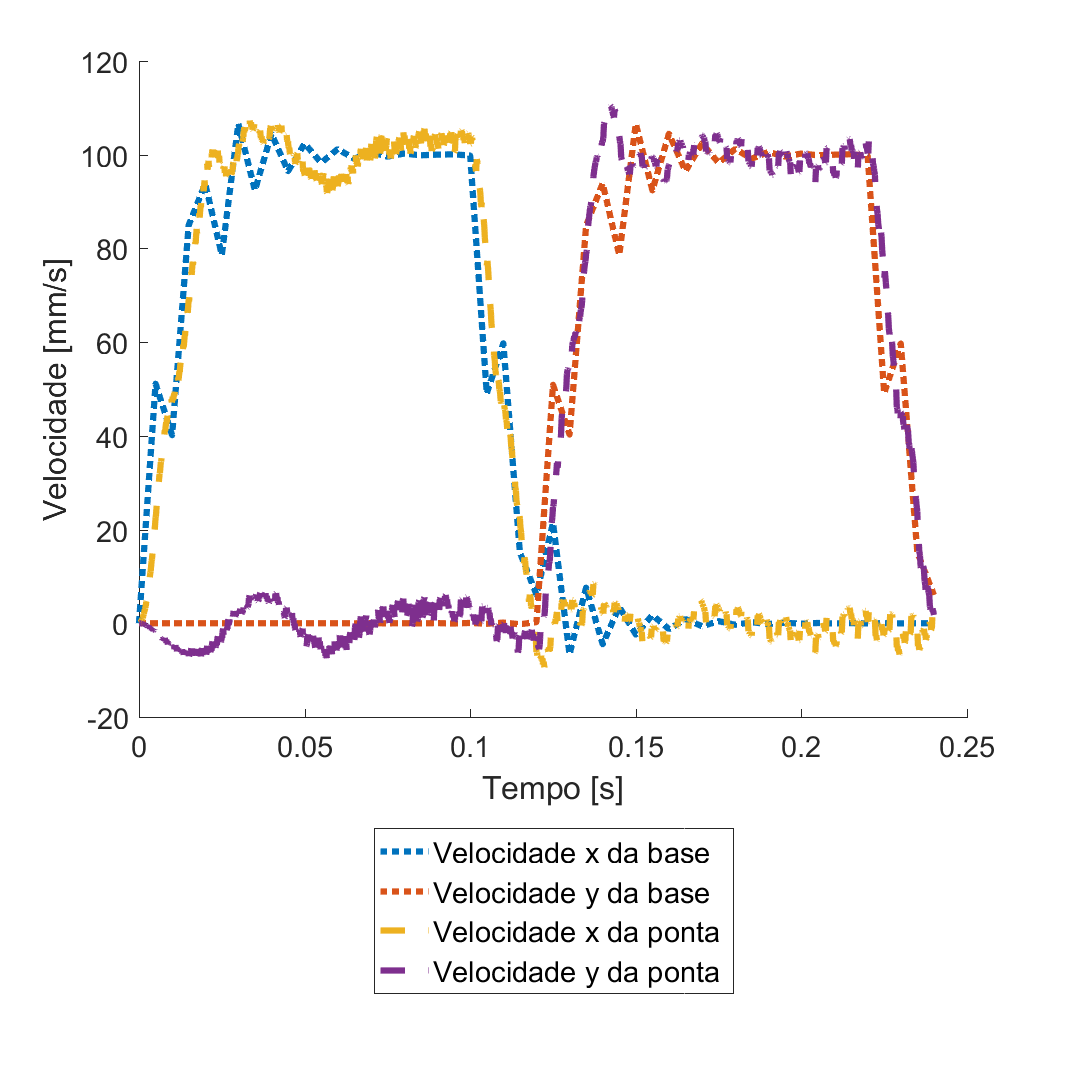
\includegraphics[width=0.47\textwidth]{Sim 1B_vel_c.png}
        \label{fig:1B_vel_c}
    }
    \caption{Velocidades da ponta e da base - Caso 1B.}
    \label{fig:1B_vel}
\end{figure}

% ------------------ end ----------------

\subsection{Caso 2 - Variação do coeficiente de amortecimento}

% ------------------ Caminho A ----------------

Apesar das grandes oscilações, a curva de deslocamento da ponta com controle não apresenta muitas dificuldades de conter essas oscilações. Em contrapartida, observa-se na Figura \ref{fig:2B_cam_p_s} que apesar do caminho da ponta sem controle se estabilizar mais rápido, o caminho da ponta com controle apresenta desvios maiores para o coeficiente de amortecimento de \(1\) (valor B).

% fig:cam
\begin{figure}[H]
    \centering
    \subfigure[Sem controle.]{
        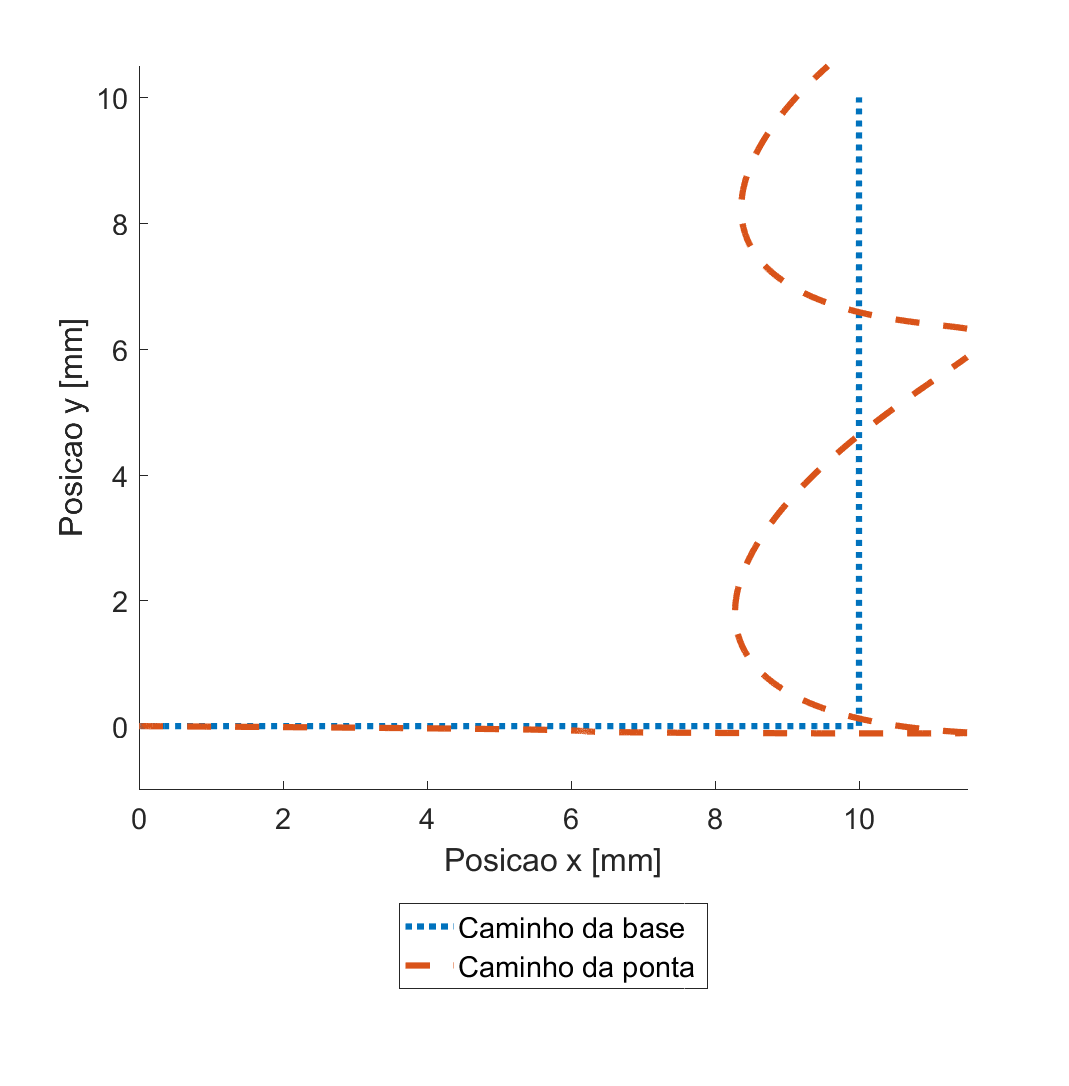
\includegraphics[width=0.47\textwidth]{Sim 2A_cam_s.png}
        \label{fig:2A_cam_s}
    }
    \hfill
    \subfigure[Com controle.]{
        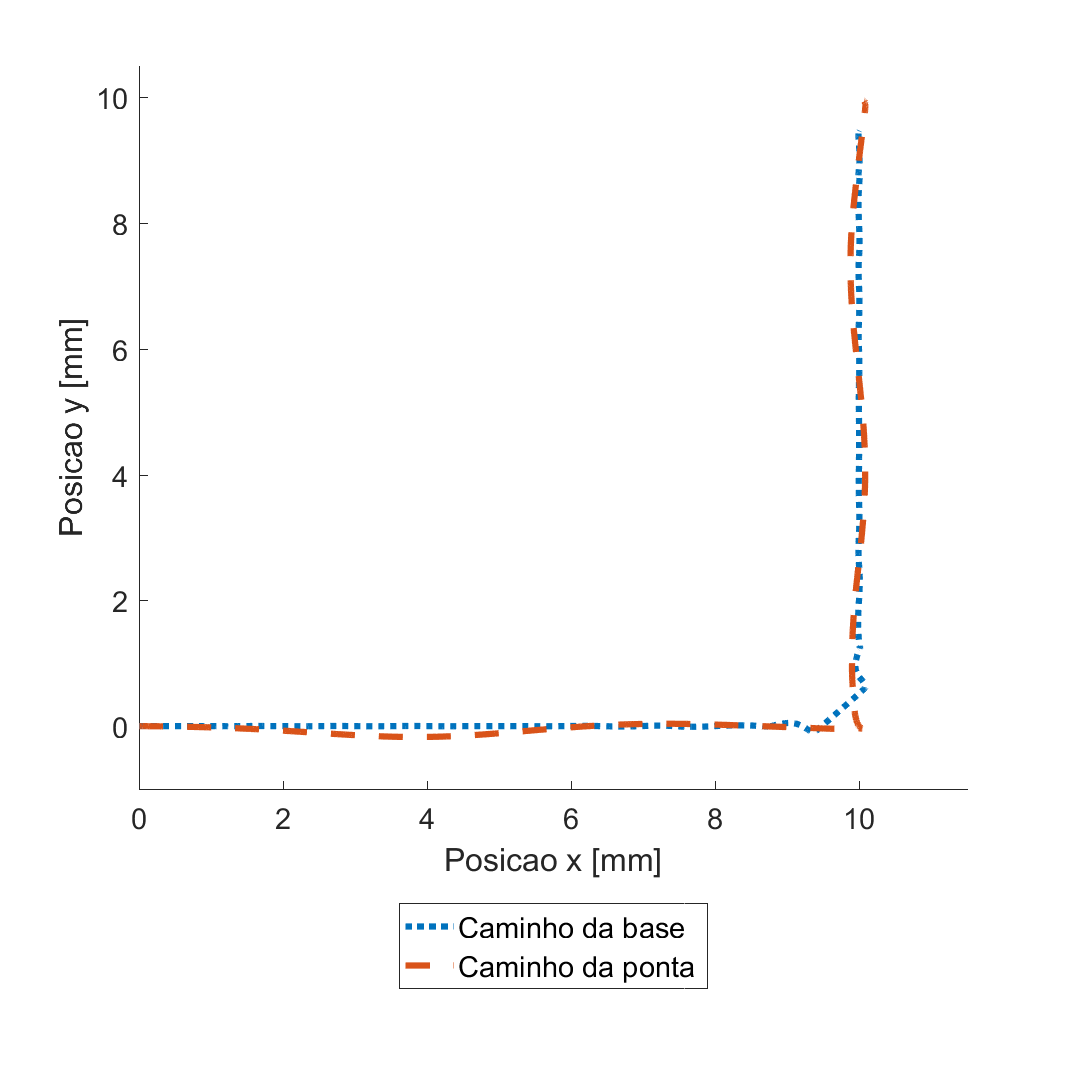
\includegraphics[width=0.47\textwidth]{Sim 2A_cam_c.png}
        \label{fig:2A_cam_c}
    }
    \hfill
    \subfigure[Detalhamento - Sem controle.]{
        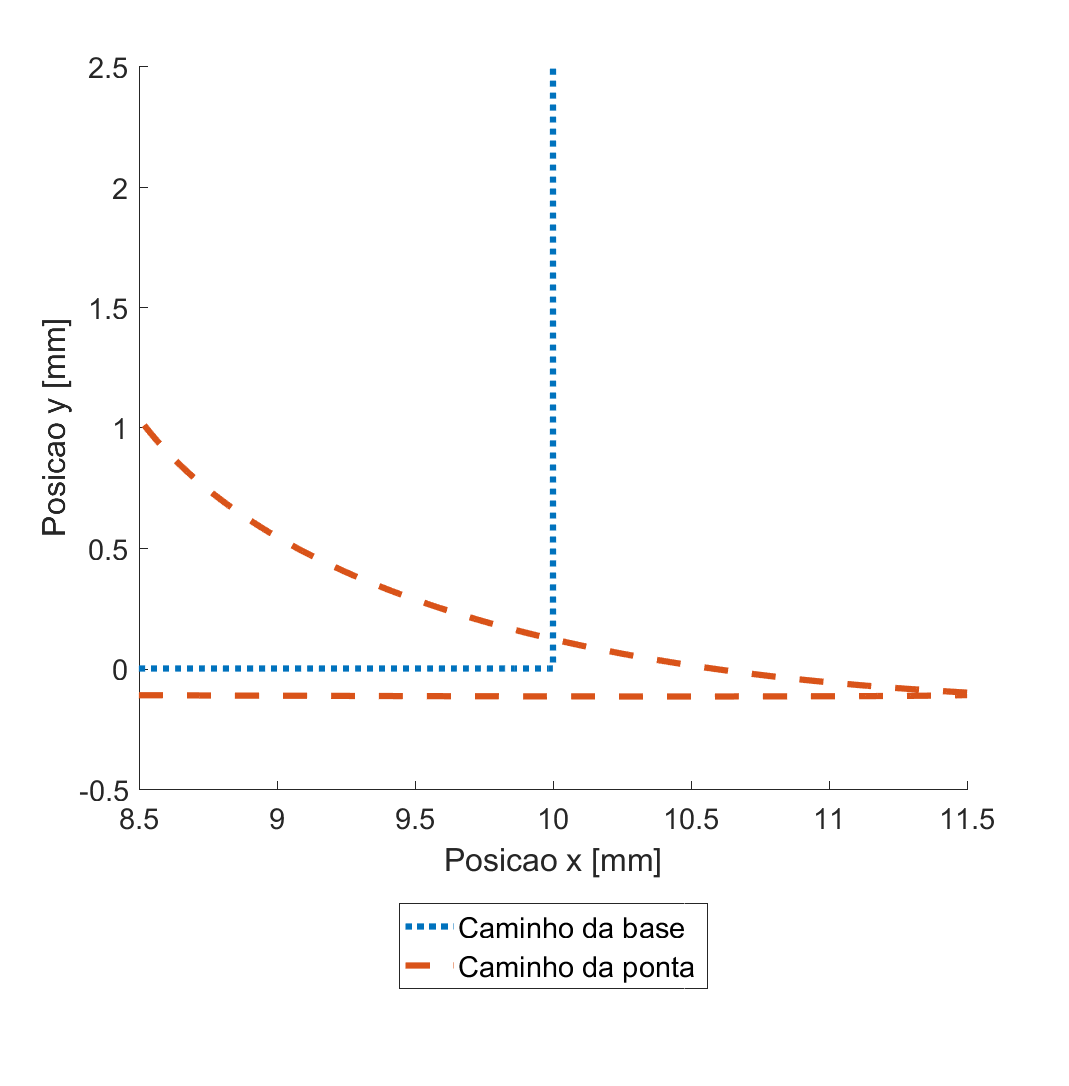
\includegraphics[width=0.47\textwidth]{Sim 2A_cam_s_zoom.png}
        \label{fig:2A_cam_s_zoom}
    }
    \hfill
    \subfigure[Detalhamento - Com controle.]{
        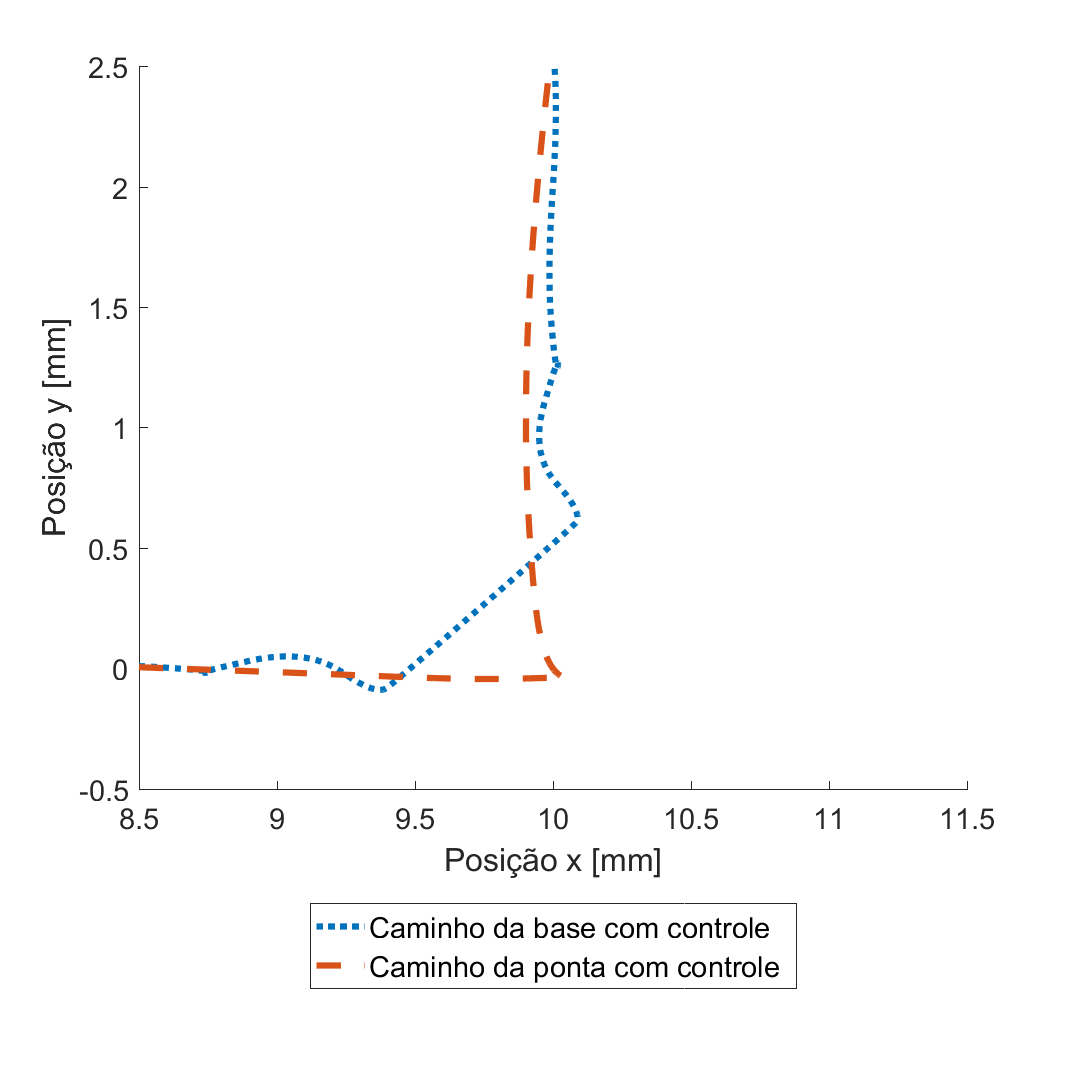
\includegraphics[width=0.47\textwidth]{Sim 2A_cam_c_zoom.png}
        \label{fig:2A_cam_c_zoom}
    }
    \caption{Caminhos da ponta e da base - Caso 2A.}
    \label{fig:2A_cam}
\end{figure}

% ------------------ Caminho B ----------------

% fig:cam
\begin{figure}[H]
    \centering
    \subfigure[Sem controle.]{
        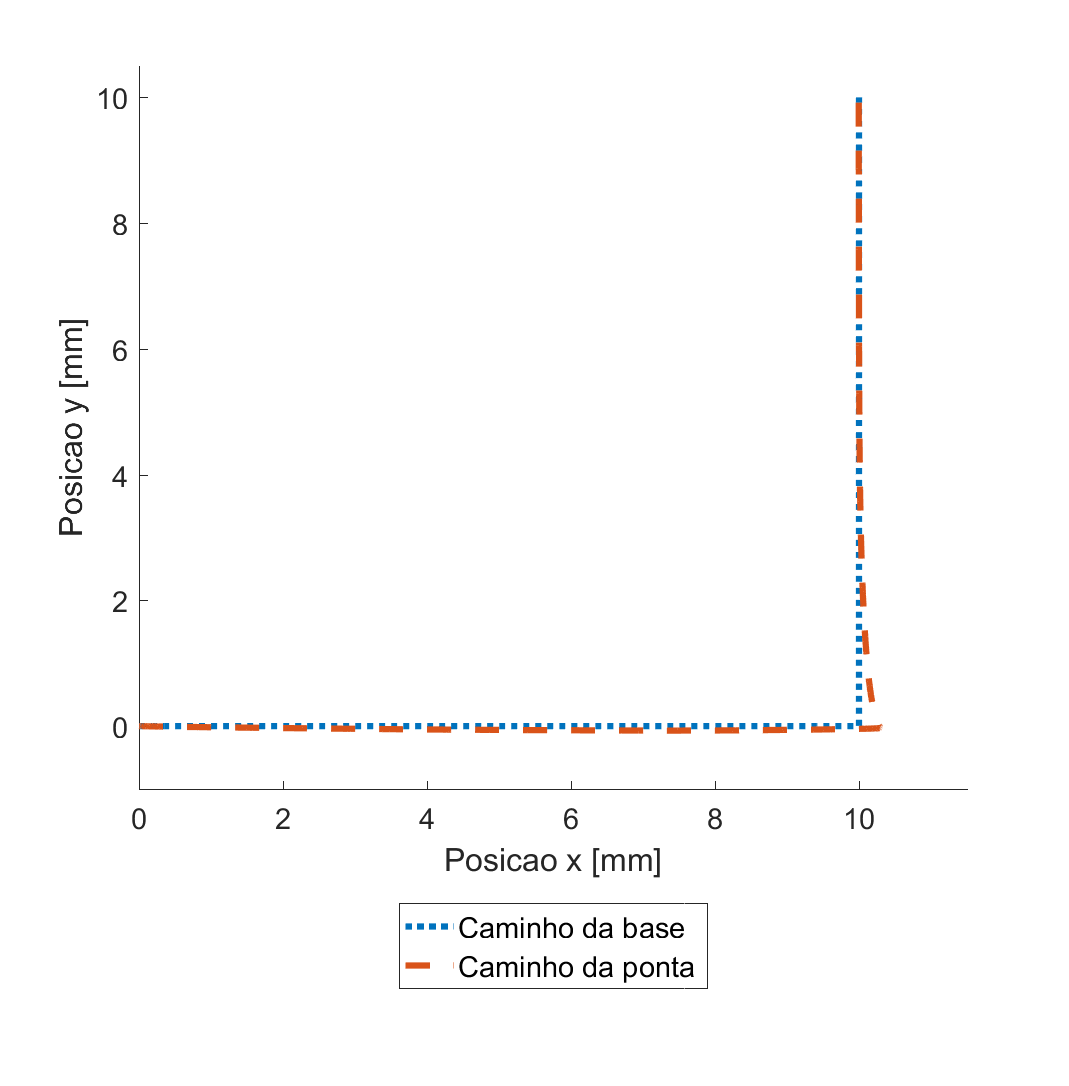
\includegraphics[width=0.47\textwidth]{Sim 2B_cam_s.png}
        \label{fig:2B_cam_s}
    }
    \hfill
    \subfigure[Com controle.]{
        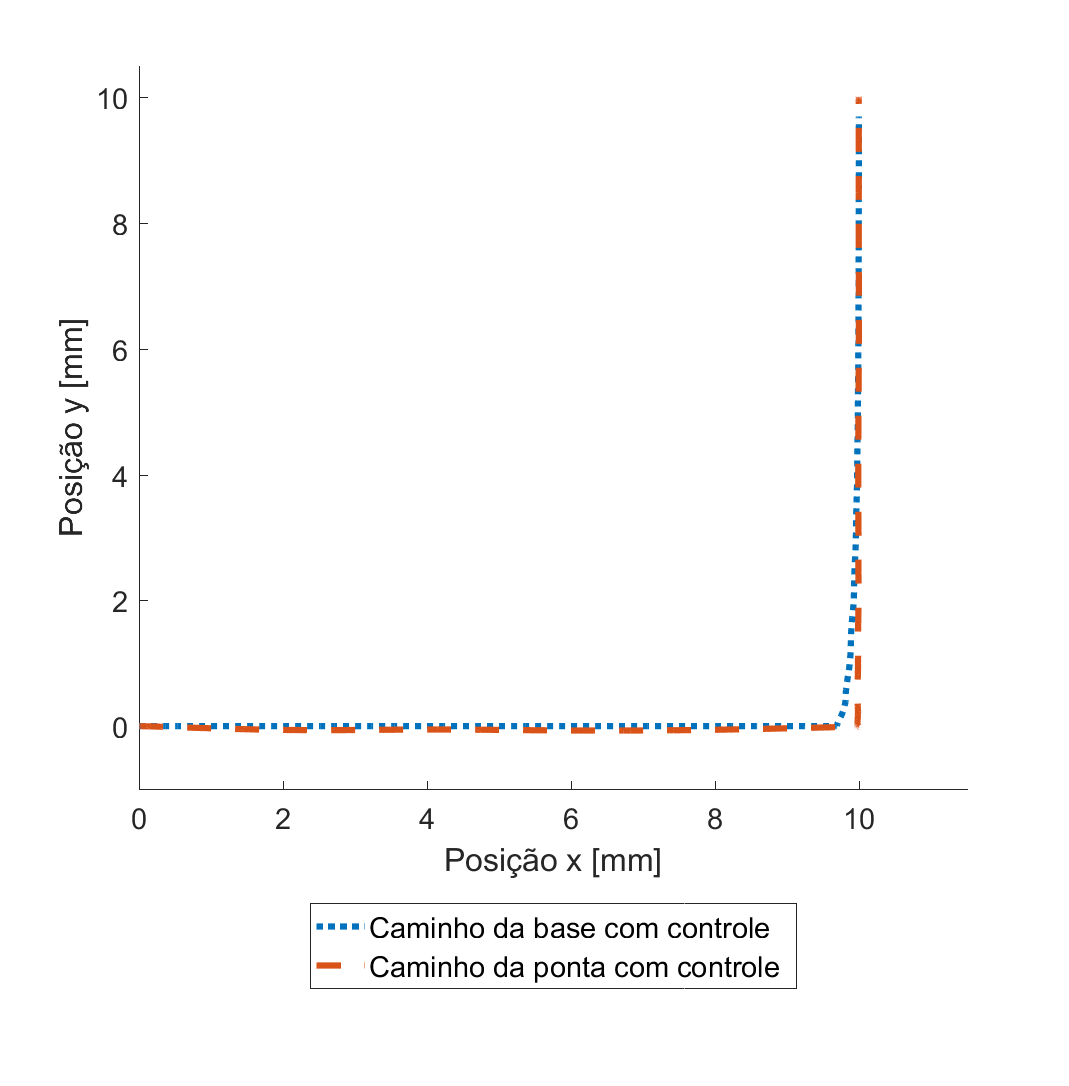
\includegraphics[width=0.47\textwidth]{Sim 2B_cam_c.png}
        \label{fig:2B_cam_c}
    }
    \hfill
    \subfigure[Detalhamento - Sem controle.]{
        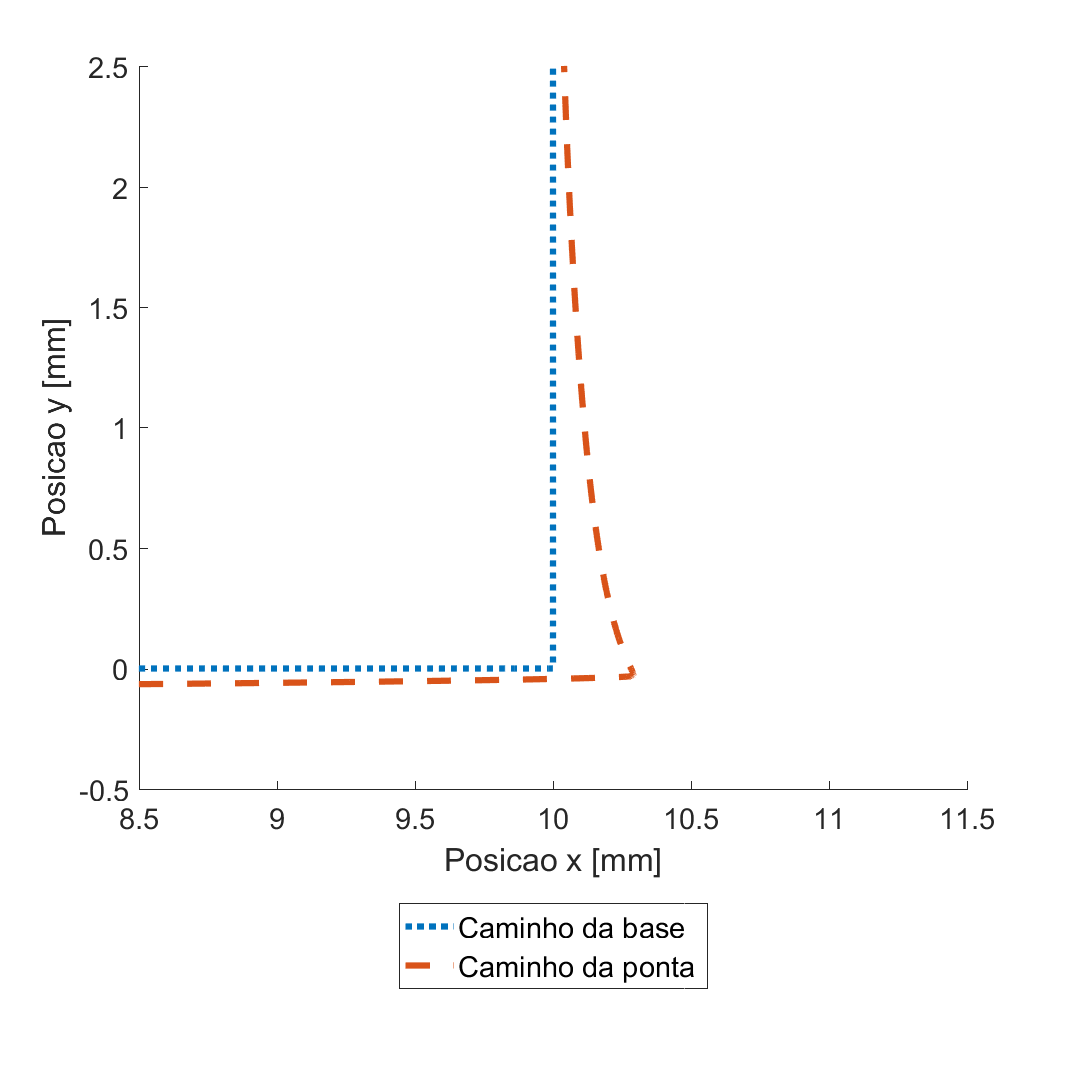
\includegraphics[width=0.47\textwidth]{Sim 2B_cam_s_zoom.png}
        \label{fig:2B_cam_s_zoom}
    }
    \hfill
    \subfigure[Detalhamento - Com controle.]{
        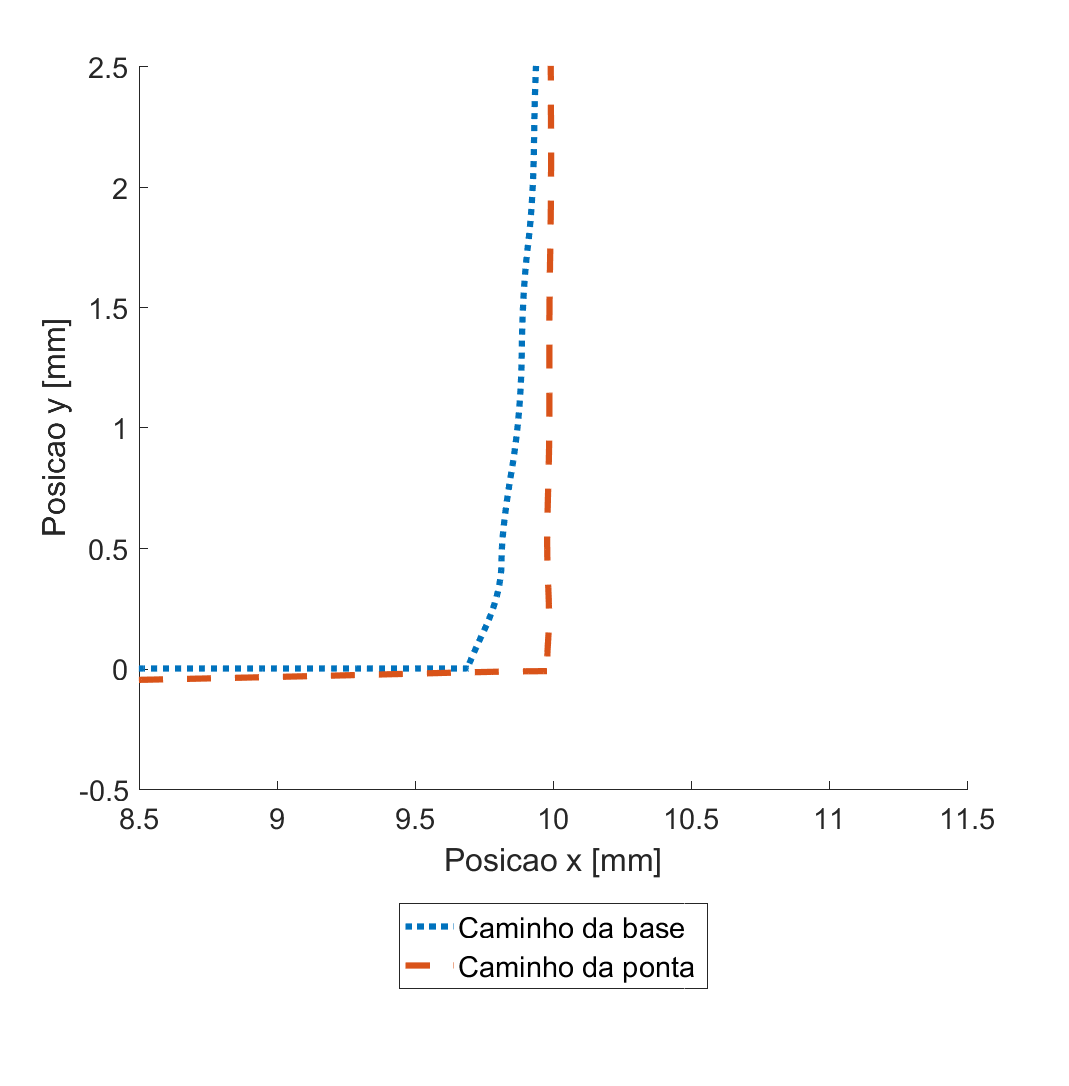
\includegraphics[width=0.47\textwidth]{Sim 2B_cam_c_zoom.png}
        \label{fig:2B_cam_c_zoom}
    }
    \caption{Caminhos da ponta e da base - Caso 2B.}
    \label{fig:2B_cam}
\end{figure}

% ------------------ Deslocamento A----------------
O principal efeito resultante da variação do coeficiente de amortecimento se dá através da característica de dissipação de energia. Nota-se na Figura \ref{fig:2A_des} a permanência das oscilações na curva de deslocamento sem controle causado pela ausência de amortecimento (valor A coeficiente de amortecimento \(0\)).

% fig:des
\begin{figure}[H]
    \centering
    \subfigure[Sem controle.]{
        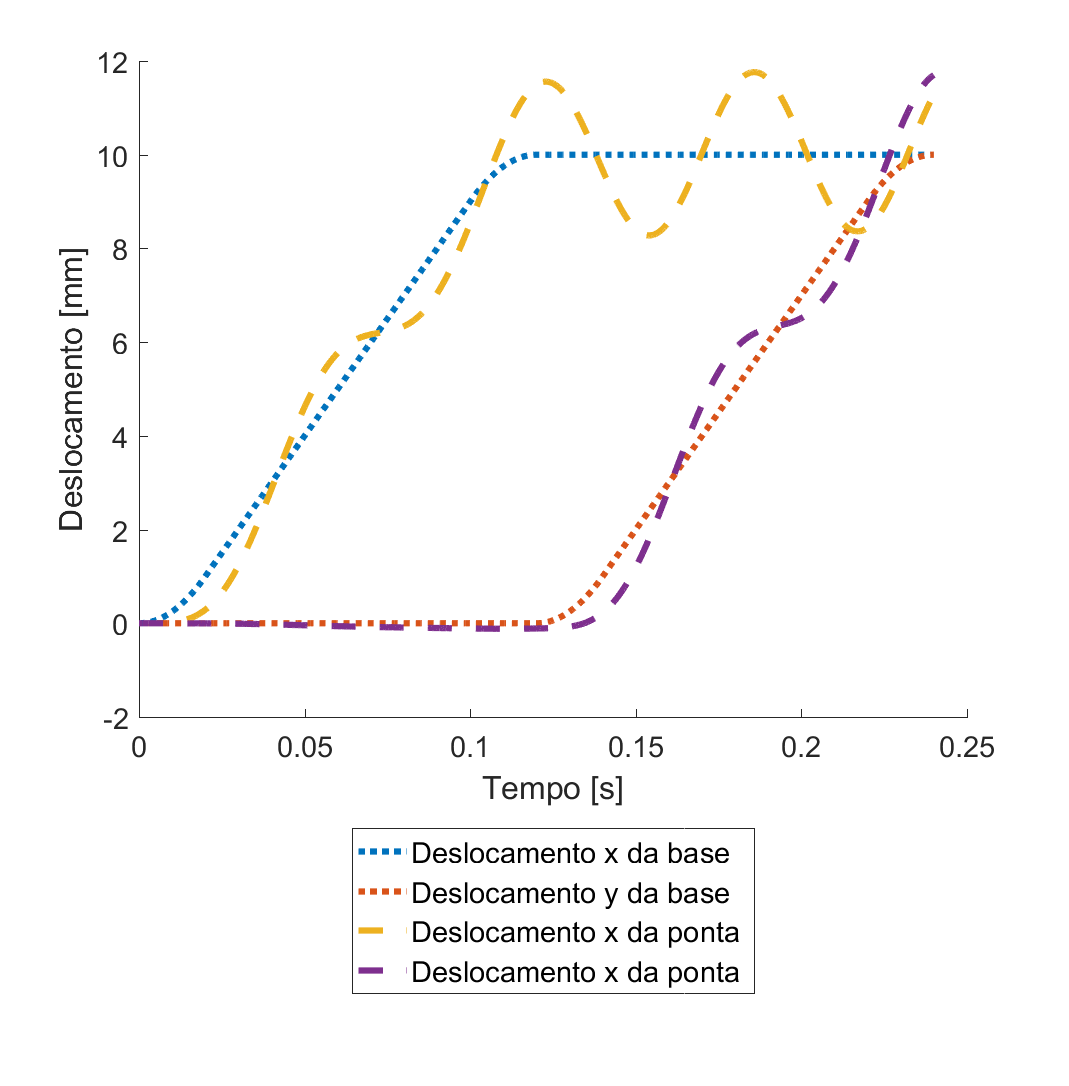
\includegraphics[width=0.47\textwidth]{Sim 2A_des_s.png}
        \label{fig:2A_des_s}
    }
    \hfill
    \subfigure[Com controle.]{
        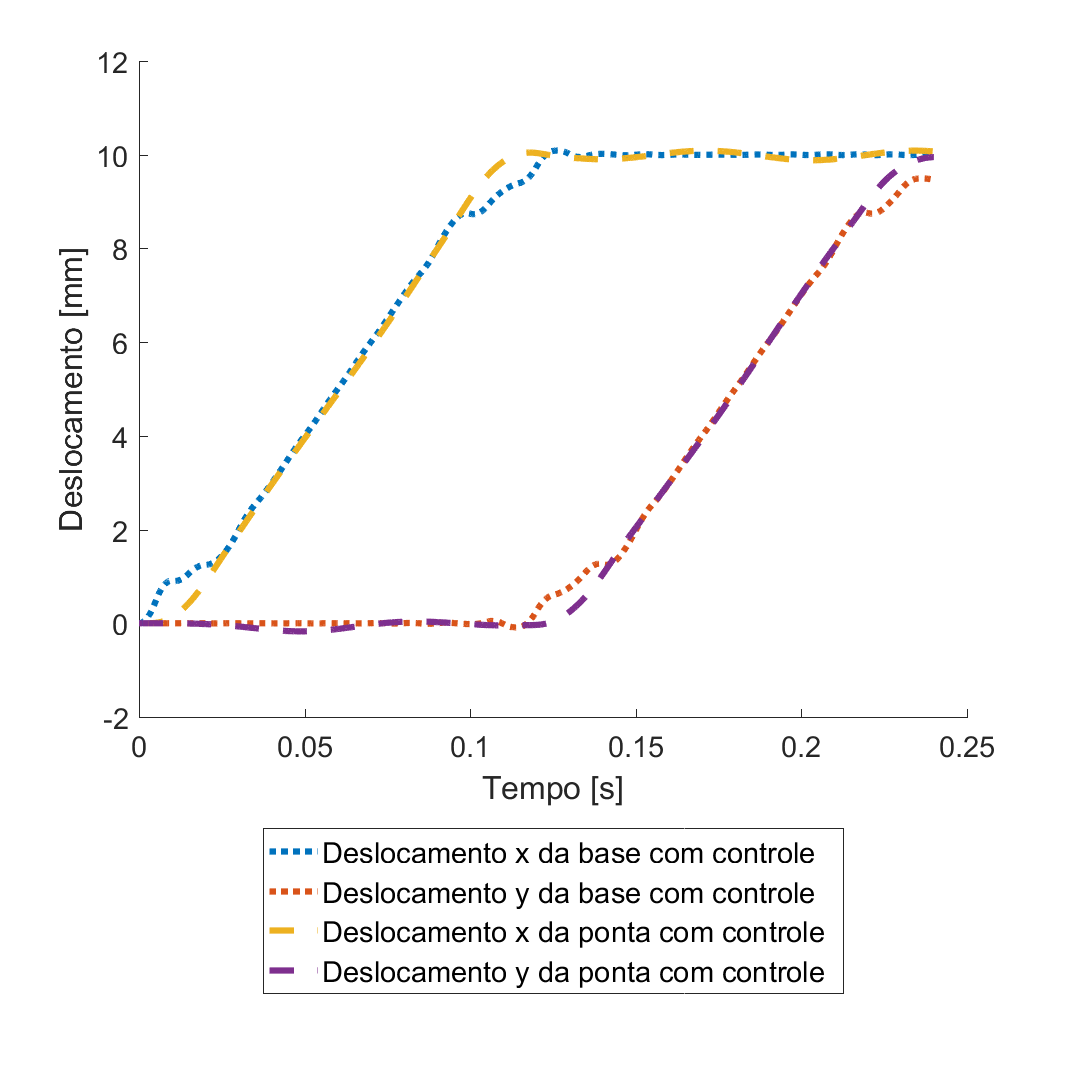
\includegraphics[width=0.47\textwidth]{Sim 2A_des_c.png}
        \label{fig:2A_des_c}
    }
    \caption{Deslocamentos da ponta e da base - Caso 2A.}
    \label{fig:2A_des}
\end{figure}

% ------------------ Deslocamento B----------------

% fig:des
\begin{figure}[H]
    \centering
    \subfigure[Sem controle.]{
        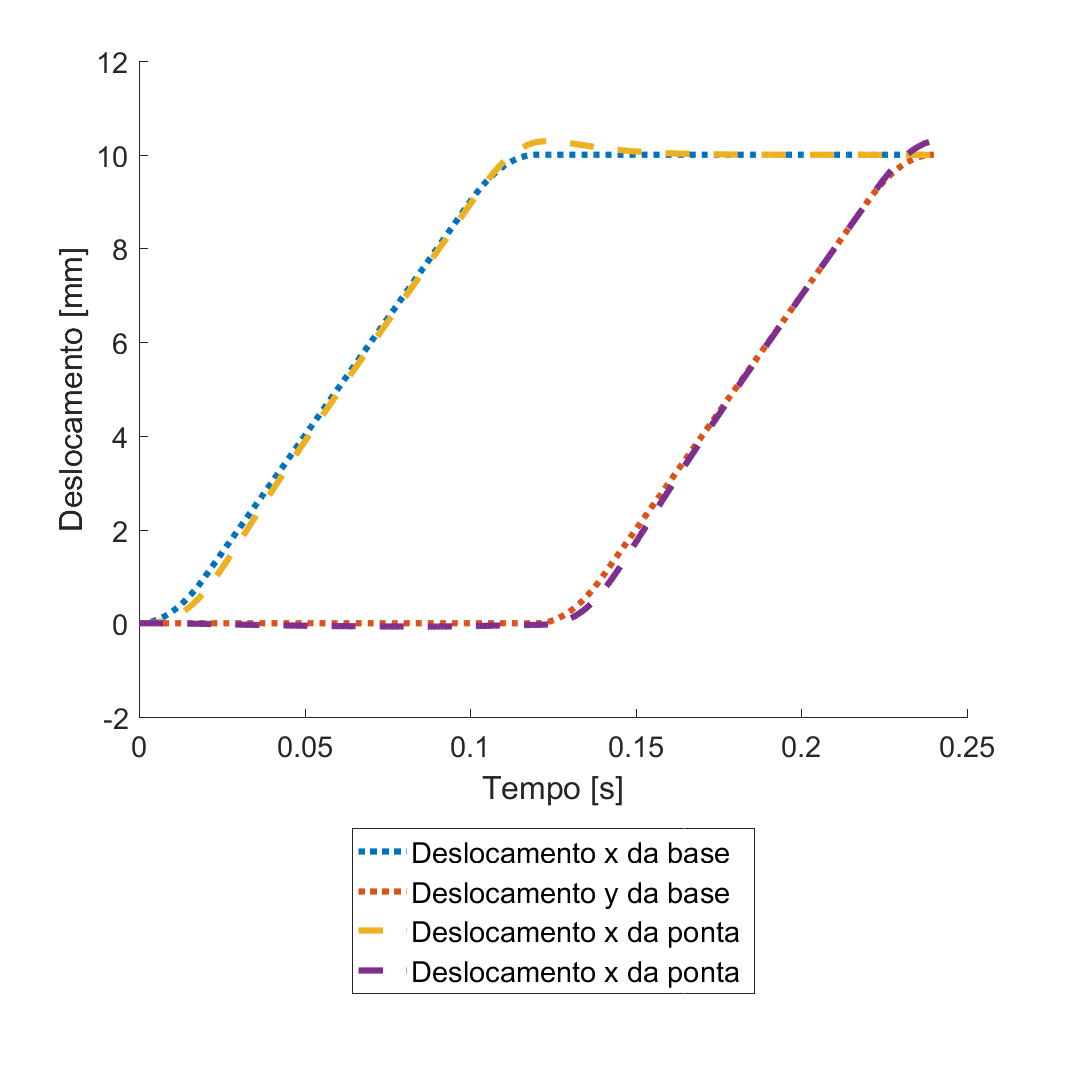
\includegraphics[width=0.47\textwidth]{Sim 2B_des_s.png}
        \label{fig:2B_des_s}
    }
    \hfill
    \subfigure[Com controle.]{
        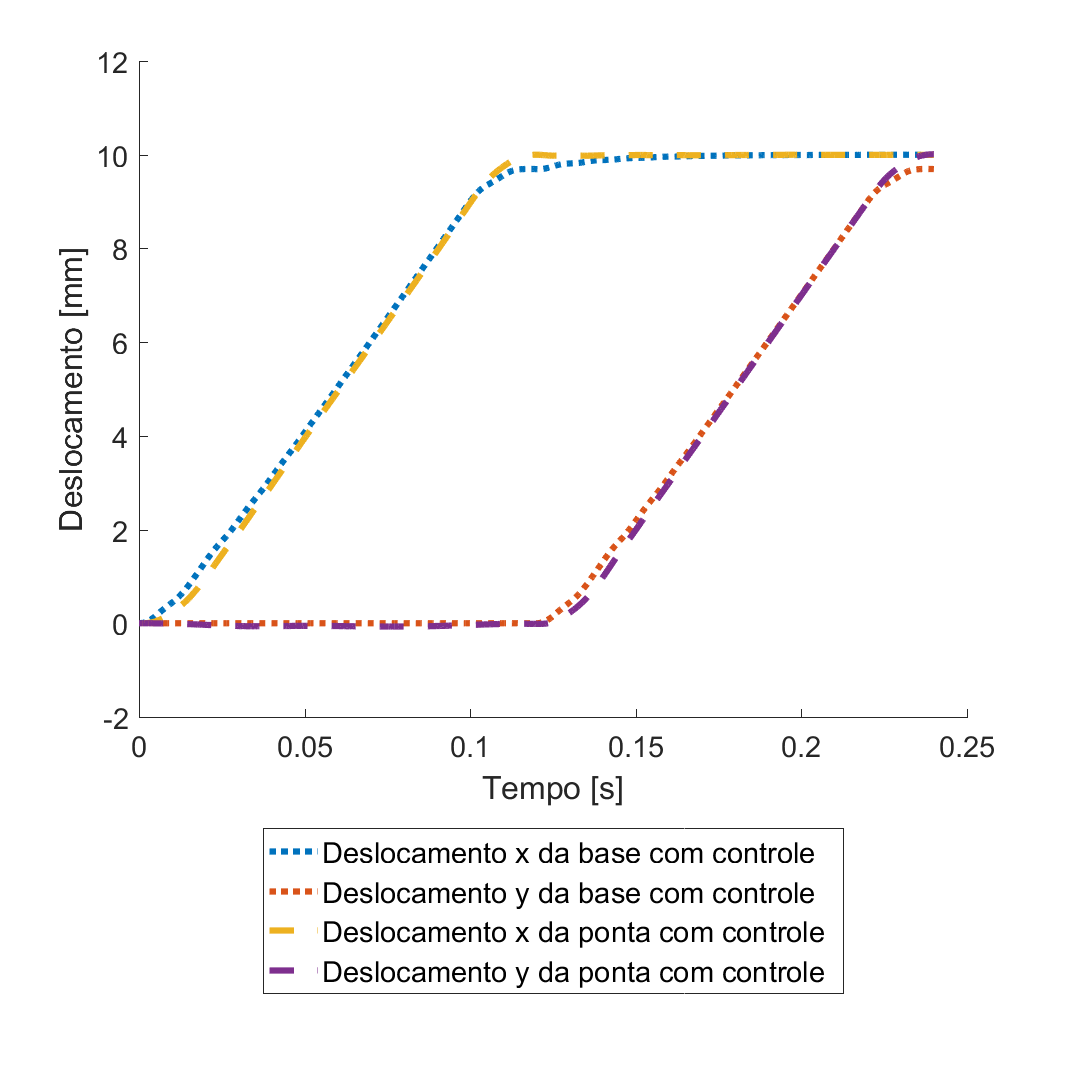
\includegraphics[width=0.47\textwidth]{Sim 2B_des_c.png}
        \label{fig:2B_des_c}
    }
    \caption{Deslocamentos da ponta e da base - Caso 2B.}
    \label{fig:2B_des}
\end{figure}

% ------------------ Velocidades A ----------------

% fig:vel
\begin{figure}[H]
    \centering
    \subfigure[Sem controle.]{
        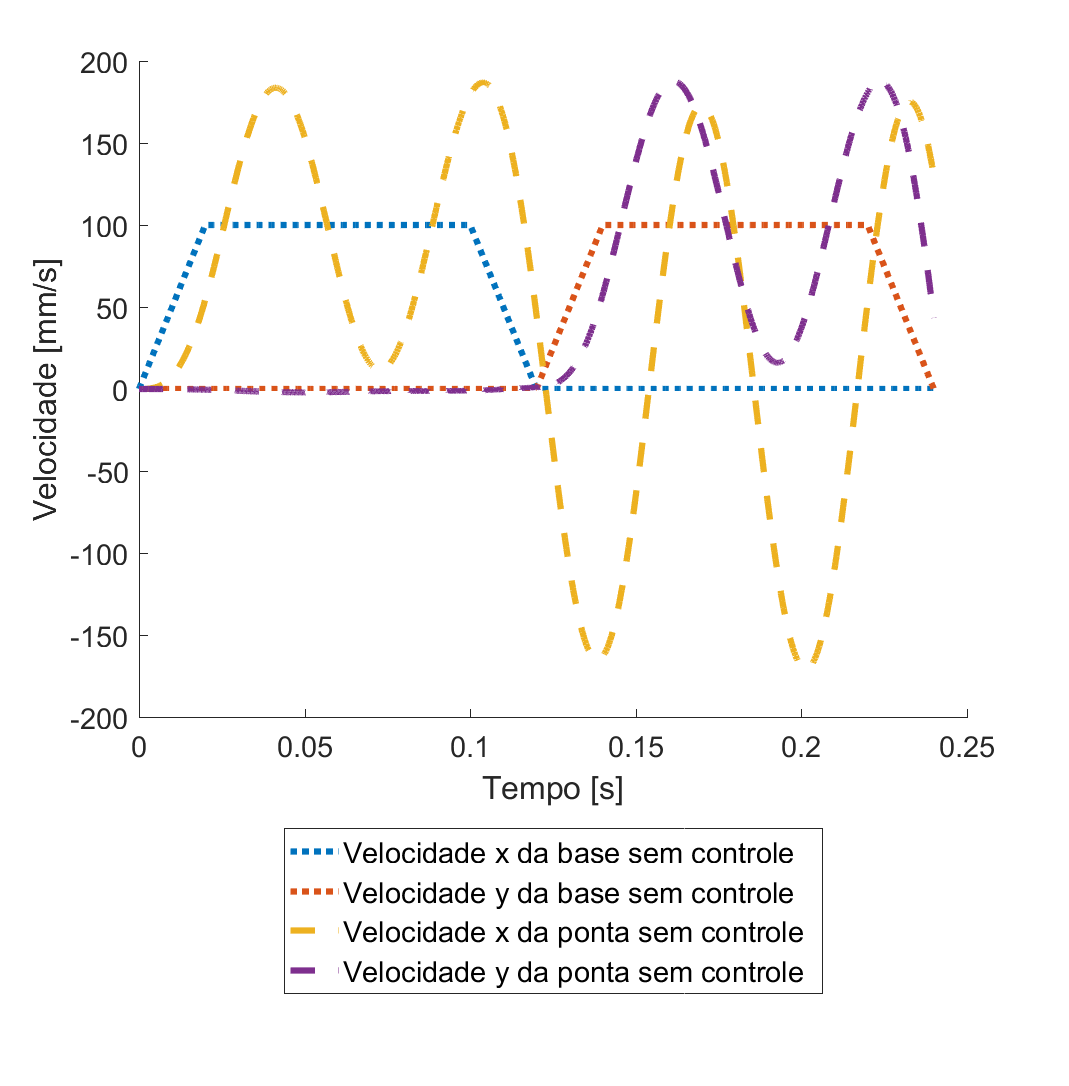
\includegraphics[width=0.47\textwidth]{Sim 2A_vel_s.png}
        \label{fig:2A_vel_s}
    }
    \hfill
    \subfigure[Com controle.]{
        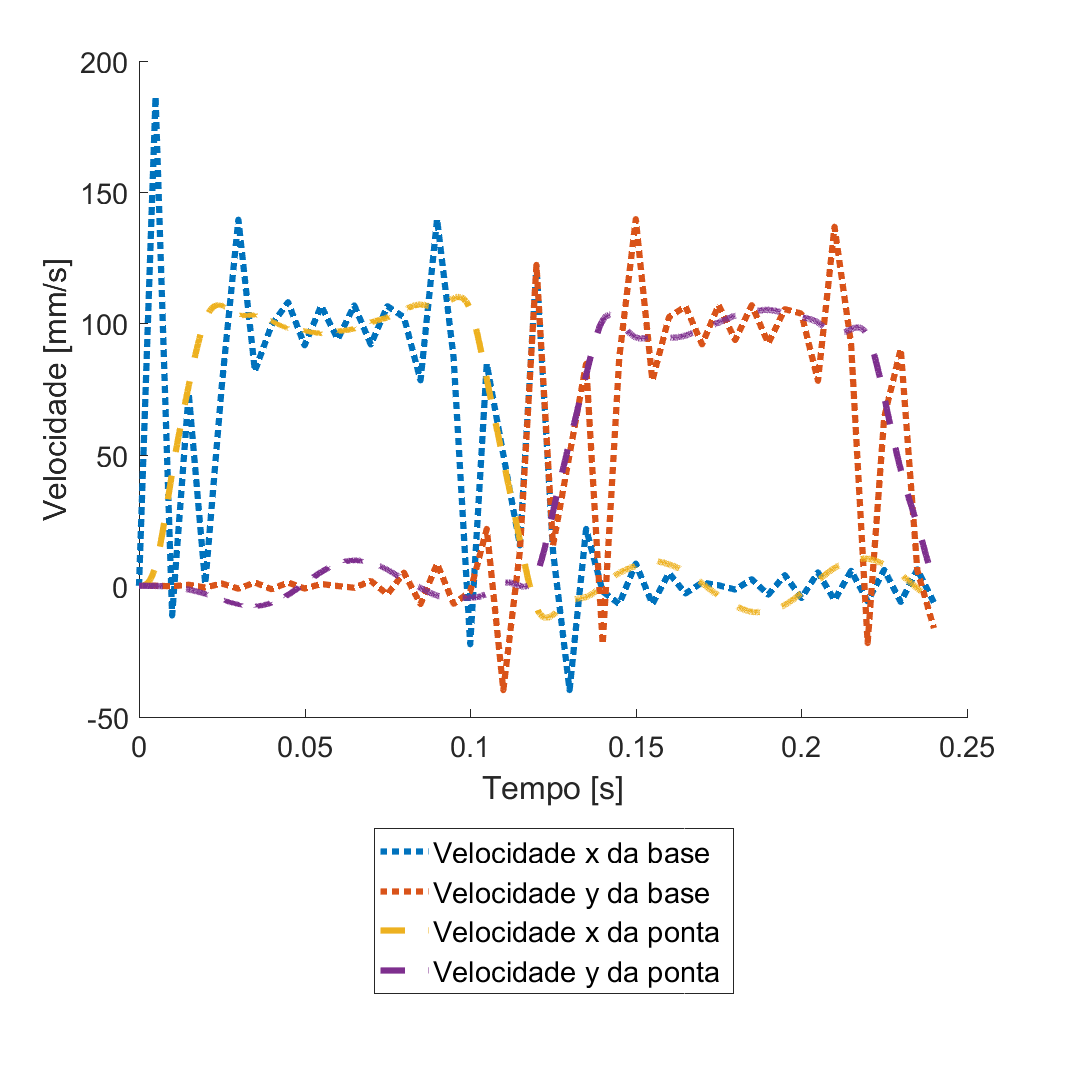
\includegraphics[width=0.47\textwidth]{Sim 2A_vel_c.png}
        \label{fig:2A_vel_c}
    }
    \caption{Velocidades da ponta e da base - Caso 2A.}
    \label{fig:2A_vel}
\end{figure}

% ------------------ Velocidades B ----------------

% fig:vel
\begin{figure}[H]
    \centering
    \subfigure[Sem controle.]{
        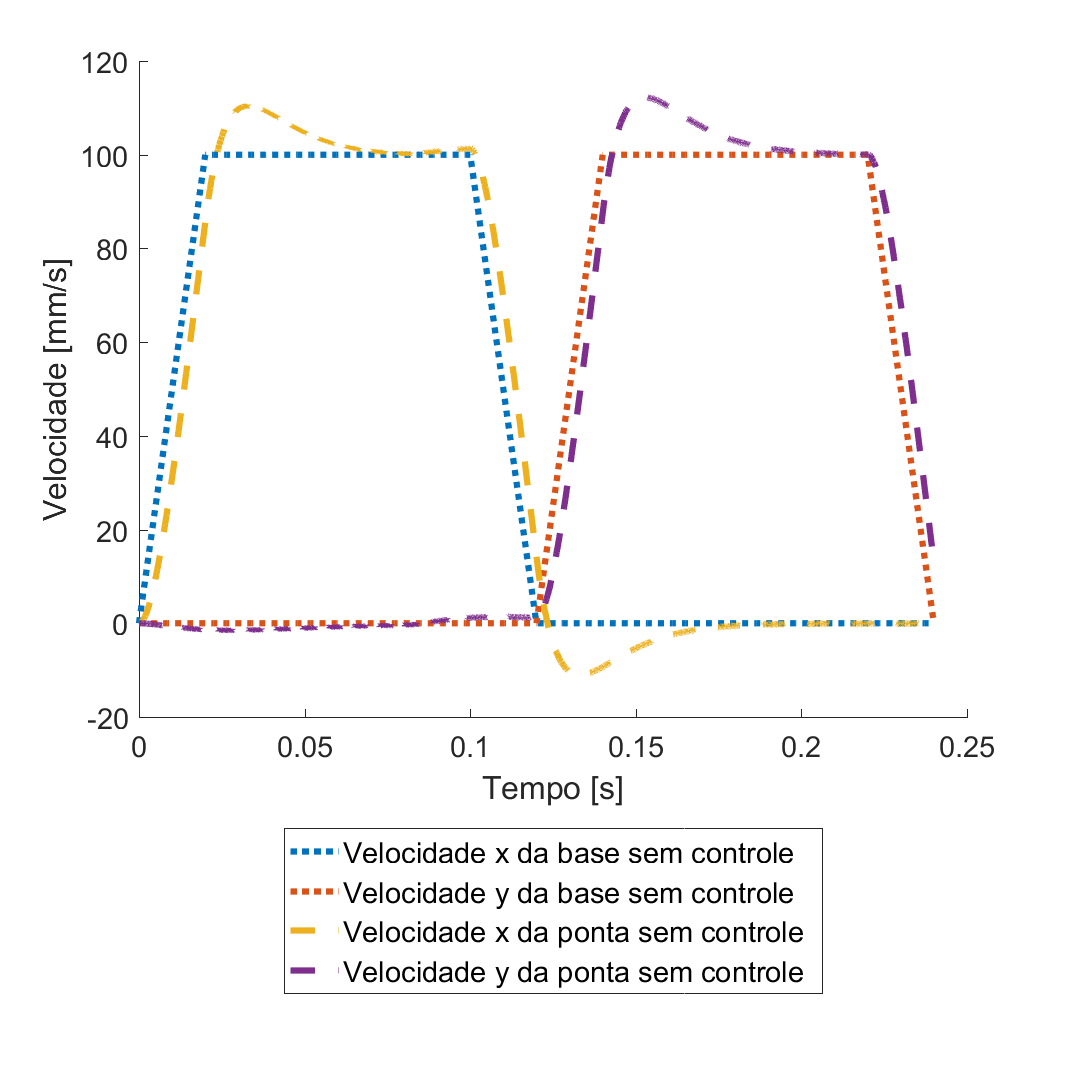
\includegraphics[width=0.47\textwidth]{Sim 2B_vel_s.png}
        \label{fig:2B_vel_s}
    }
    \hfill
    \subfigure[Com controle.]{
        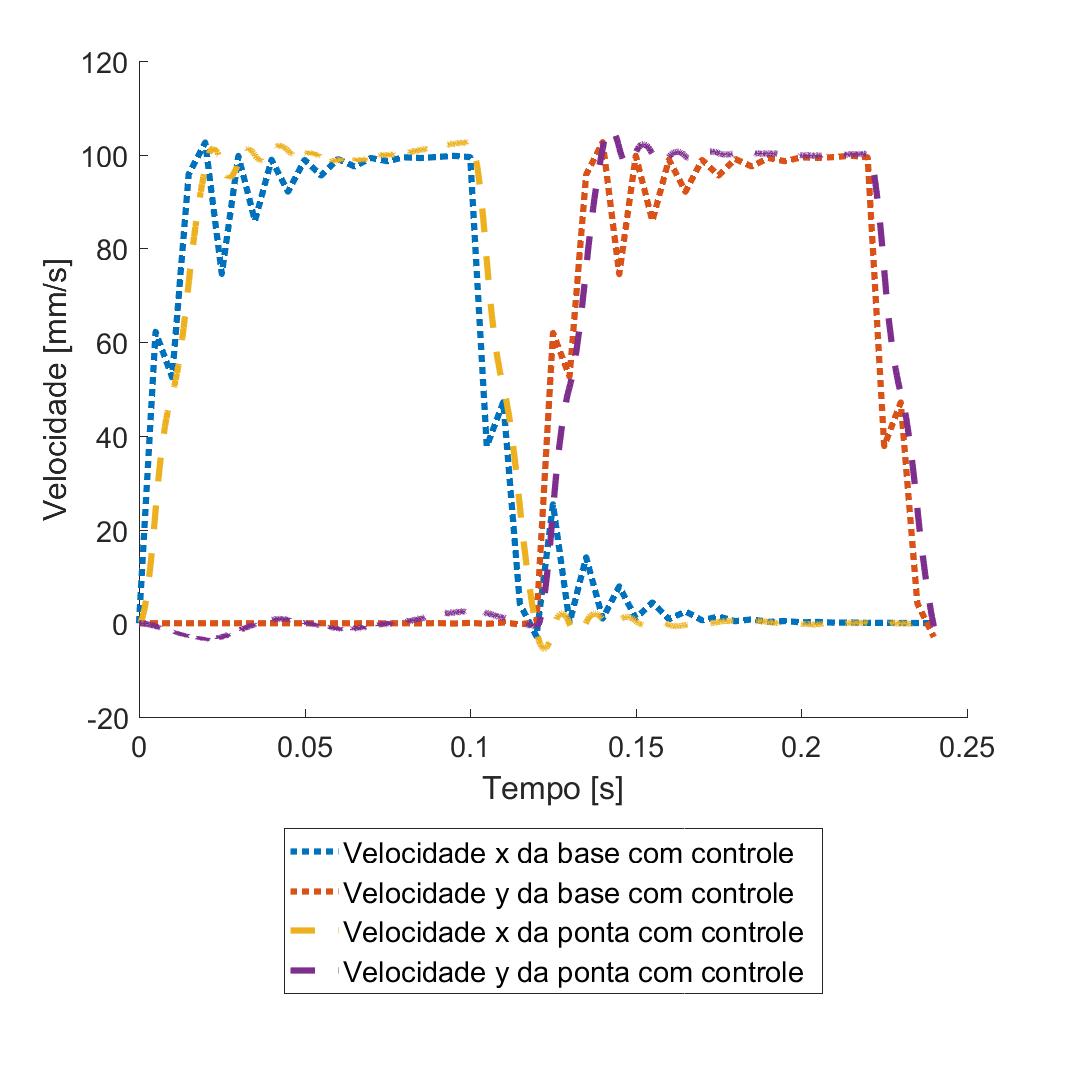
\includegraphics[width=0.47\textwidth]{Sim 2B_vel_c.png}
        \label{fig:2B_vel_c}
    }
    \caption{Velocidades da ponta e da base - Caso 2B.}
    \label{fig:2B_vel}
\end{figure}

% ------------------ end ----------------


\subsection{Caso 3 - Variação na aceleração}

% ------------------ Caminho A ----------------

Além disso, os efeitos deste parâmetro também afetam o sobre-sinal e velocidade média, de maneira que maiores acelerações proporcionam menores tempos de impressão, em contrapartida maiores oscilações e maior sobre-sinal. Assim como menores acelerações, maior tempo de impressão e menores oscilações. Em contrapartida, observa-se a atuação do controle de trajetória em minimizar os desvios de caminho da curva de maior aceleração, melhorando a balança entre velocidade e desvios se comparado à curva de menor aceleração. Estes efeitos são ilustrados nas Figuras \ref{fig:3A_cam_p_s} e \ref{fig:3B_cam_p_s}, para os valores A e B respectivamente.

% fig:cam
\begin{figure}[H]
    \centering
    \subfigure[Sem controle.]{
        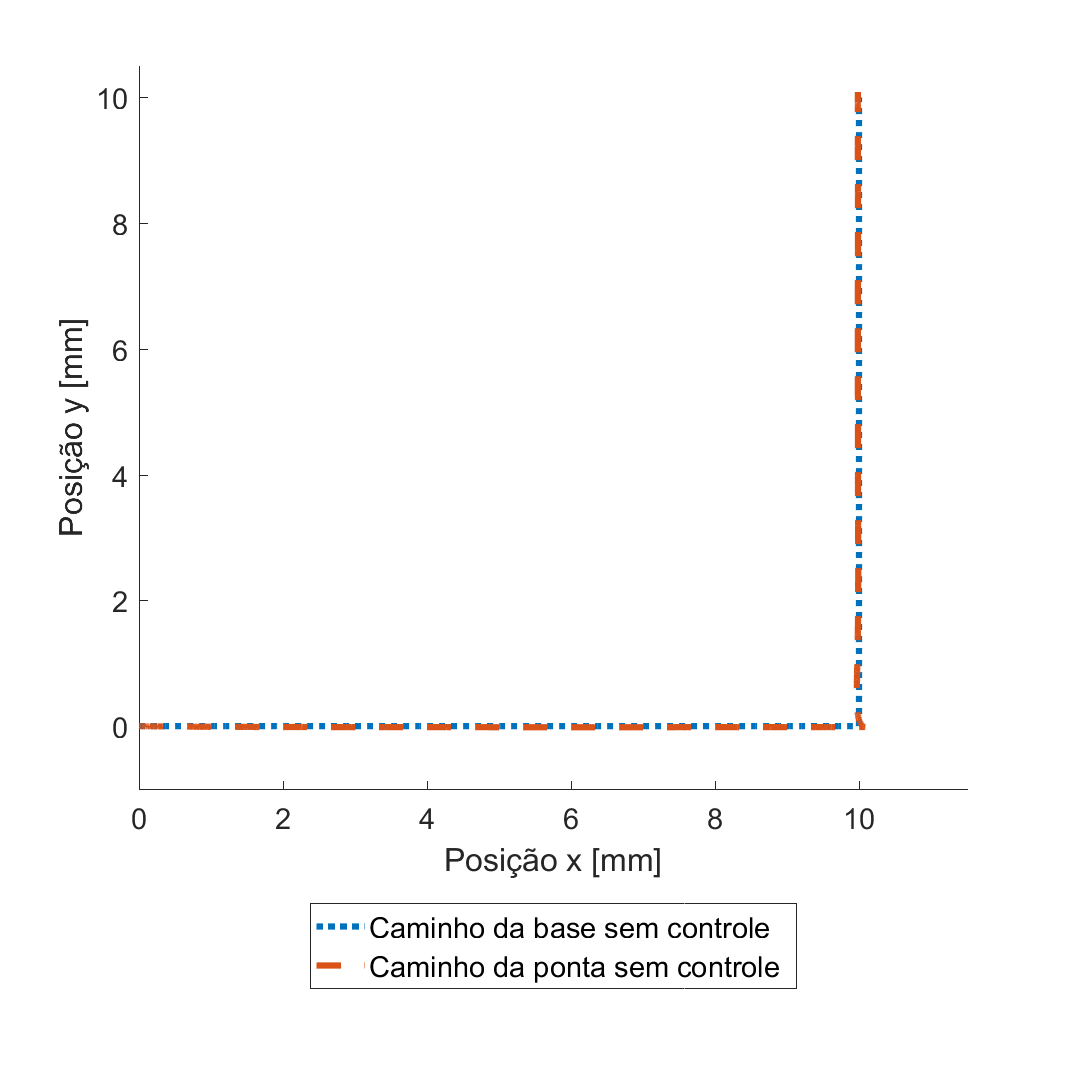
\includegraphics[width=0.47\textwidth]{Sim 3A_cam_s.png}
        \label{fig:3A_cam_s}
    }
    \hfill
    \subfigure[Com controle.]{
        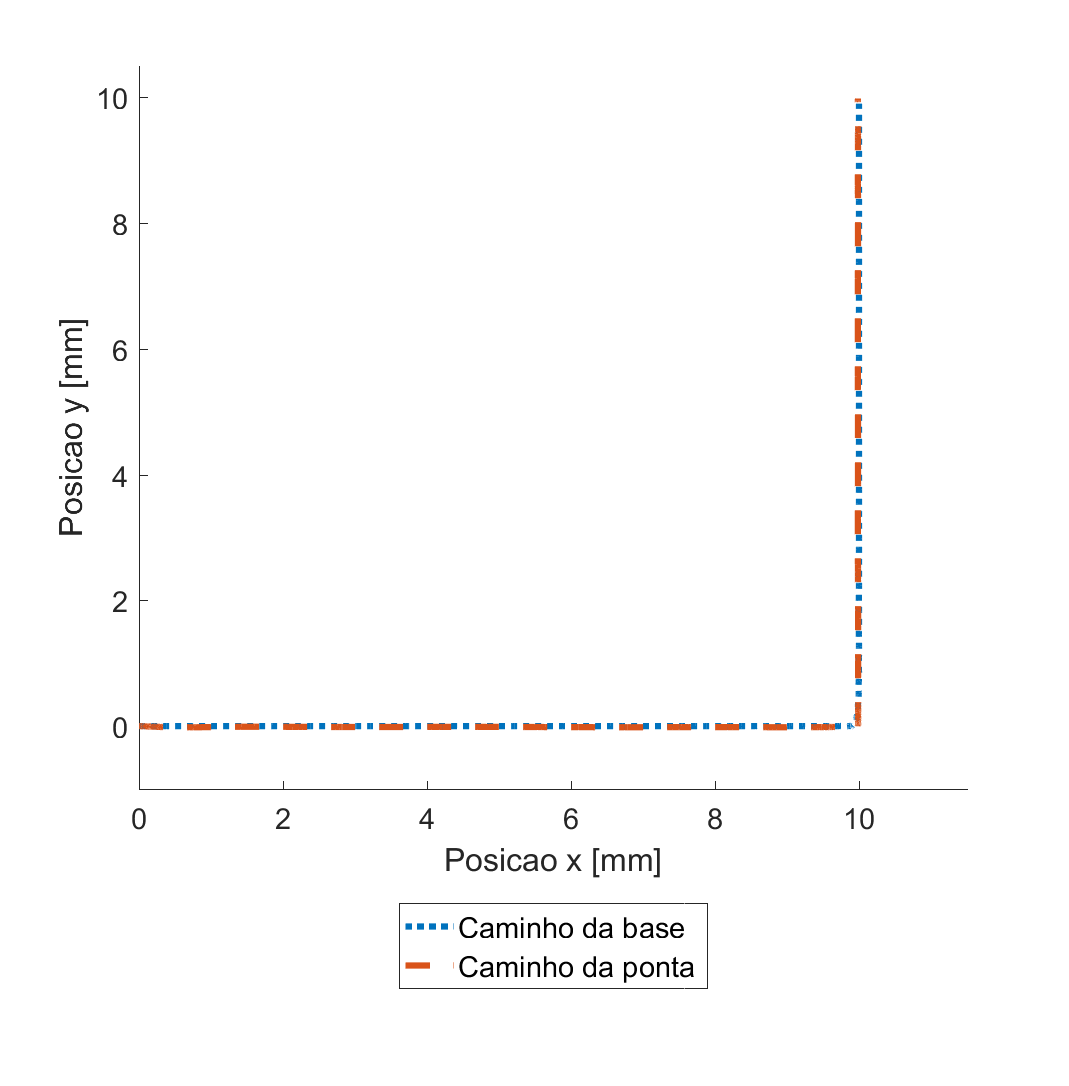
\includegraphics[width=0.47\textwidth]{Sim 3A_cam_c.png}
        \label{fig:3A_cam_c}
    }
    \hfill
    \subfigure[Detalhamento - Sem controle.]{
        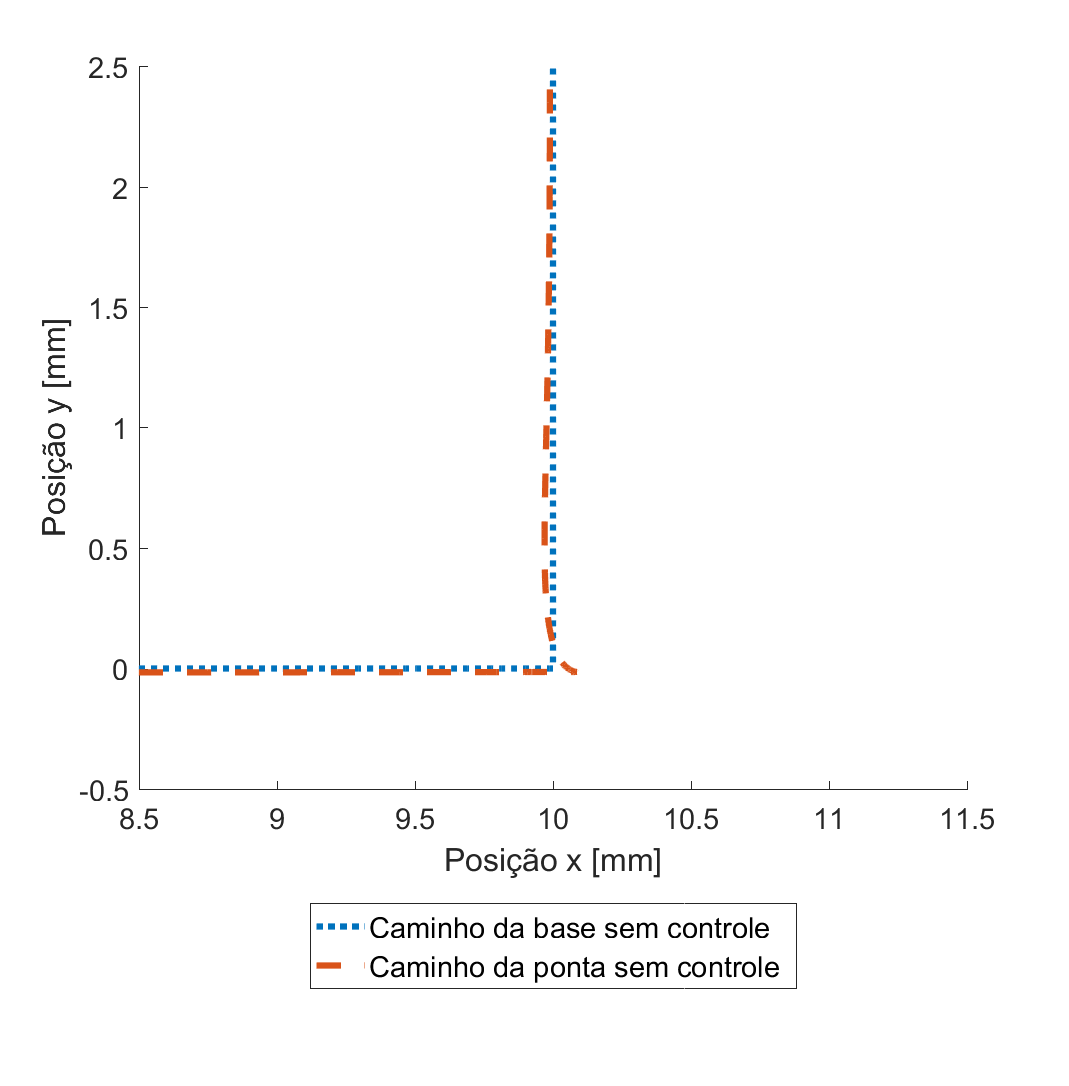
\includegraphics[width=0.47\textwidth]{Sim 3A_cam_s_zoom.png}
        \label{fig:3A_cam_s_zoom}
    }
    \hfill
    \subfigure[Detalhamento - Com controle.]{
        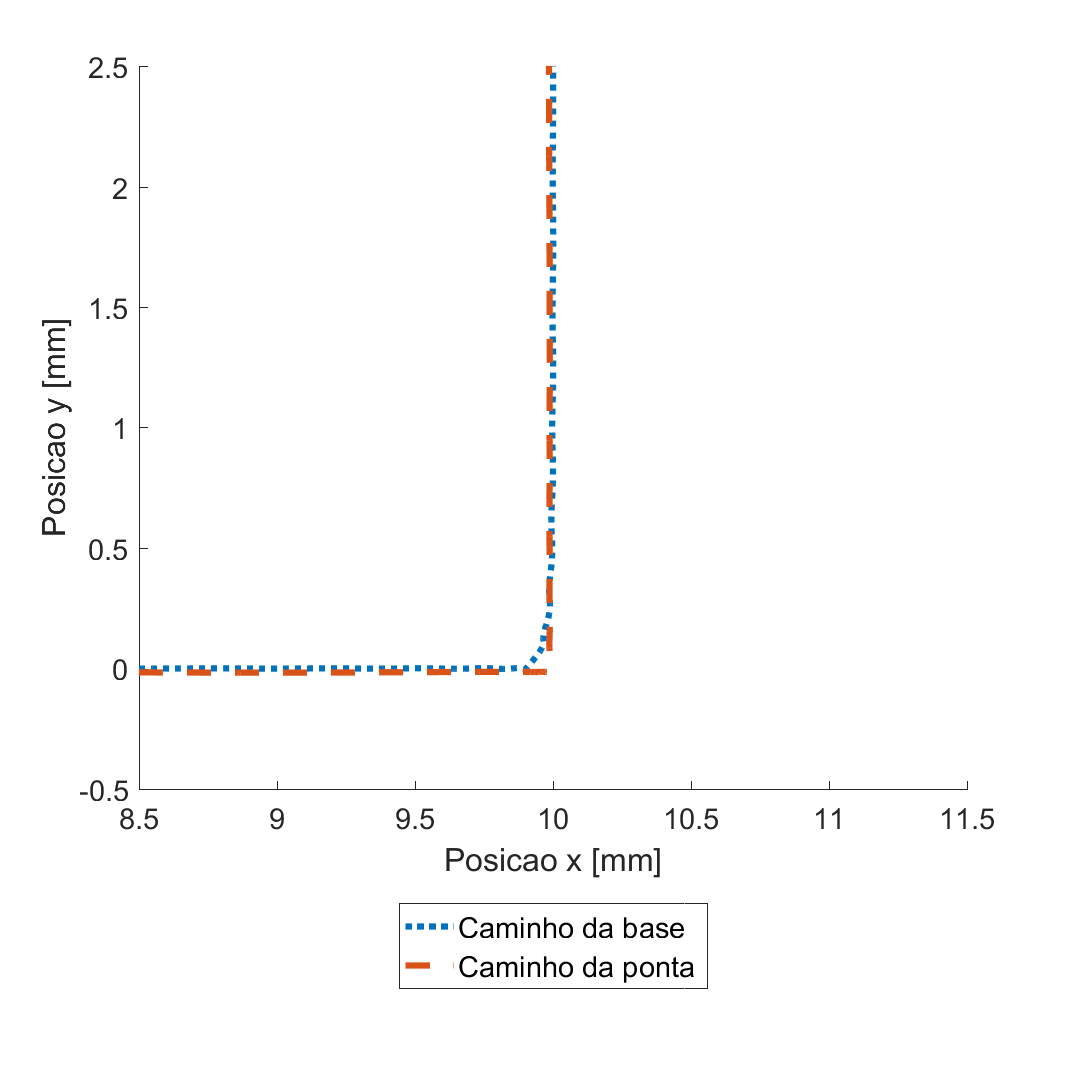
\includegraphics[width=0.47\textwidth]{Sim 3A_cam_c_zoom.png}
        \label{fig:3A_cam_c_zoom}
    }
    \caption{Caminhos da ponta e da base - Caso 3A.}
    \label{fig:3A_cam}
\end{figure}

% ------------------ Caminho B ----------------

% fig:cam
\begin{figure}[H]
    \centering
    \subfigure[Sem controle.]{
        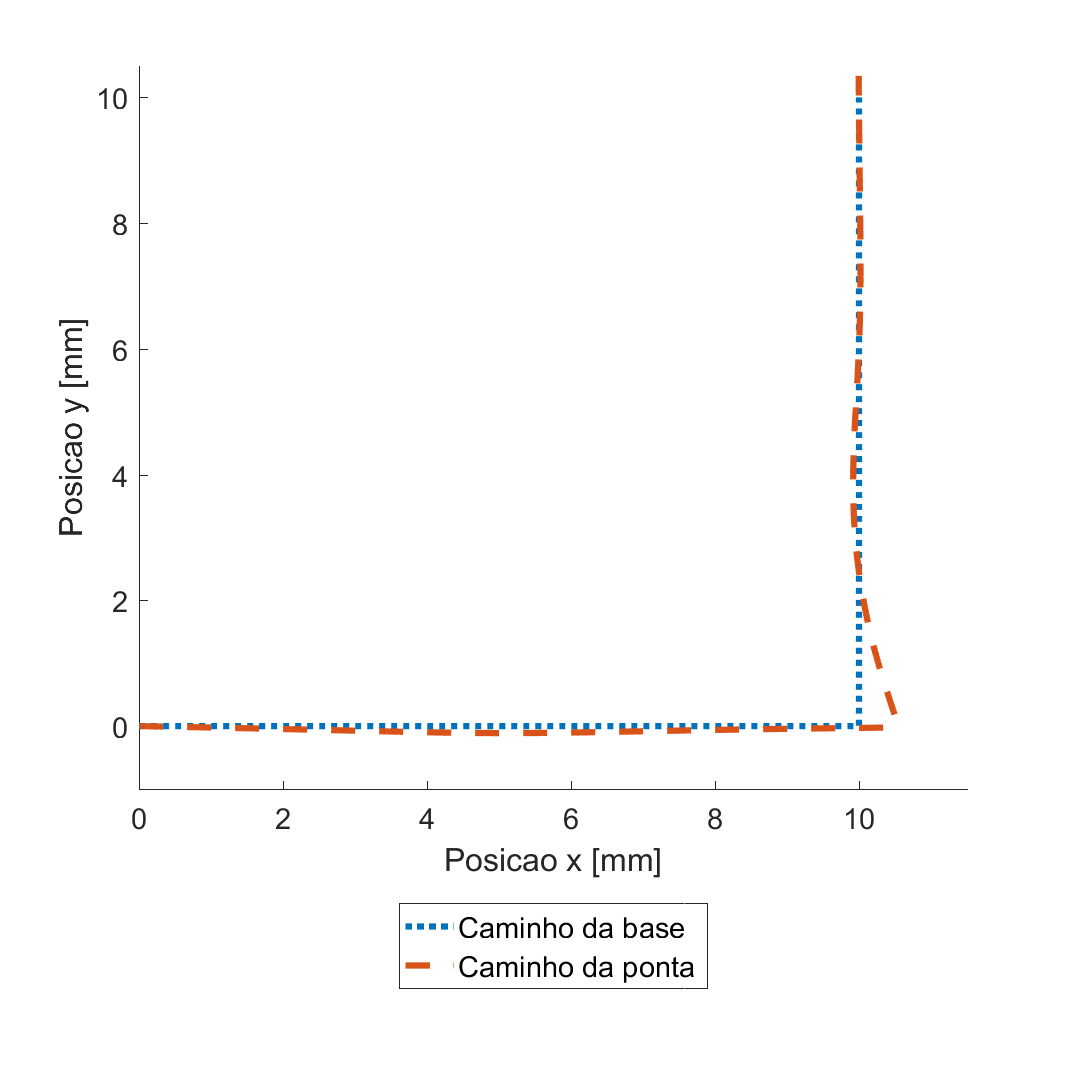
\includegraphics[width=0.47\textwidth]{Sim 3B_cam_s.png}
        \label{fig:3B_cam_s}
    }
    \hfill
    \subfigure[Com controle.]{
        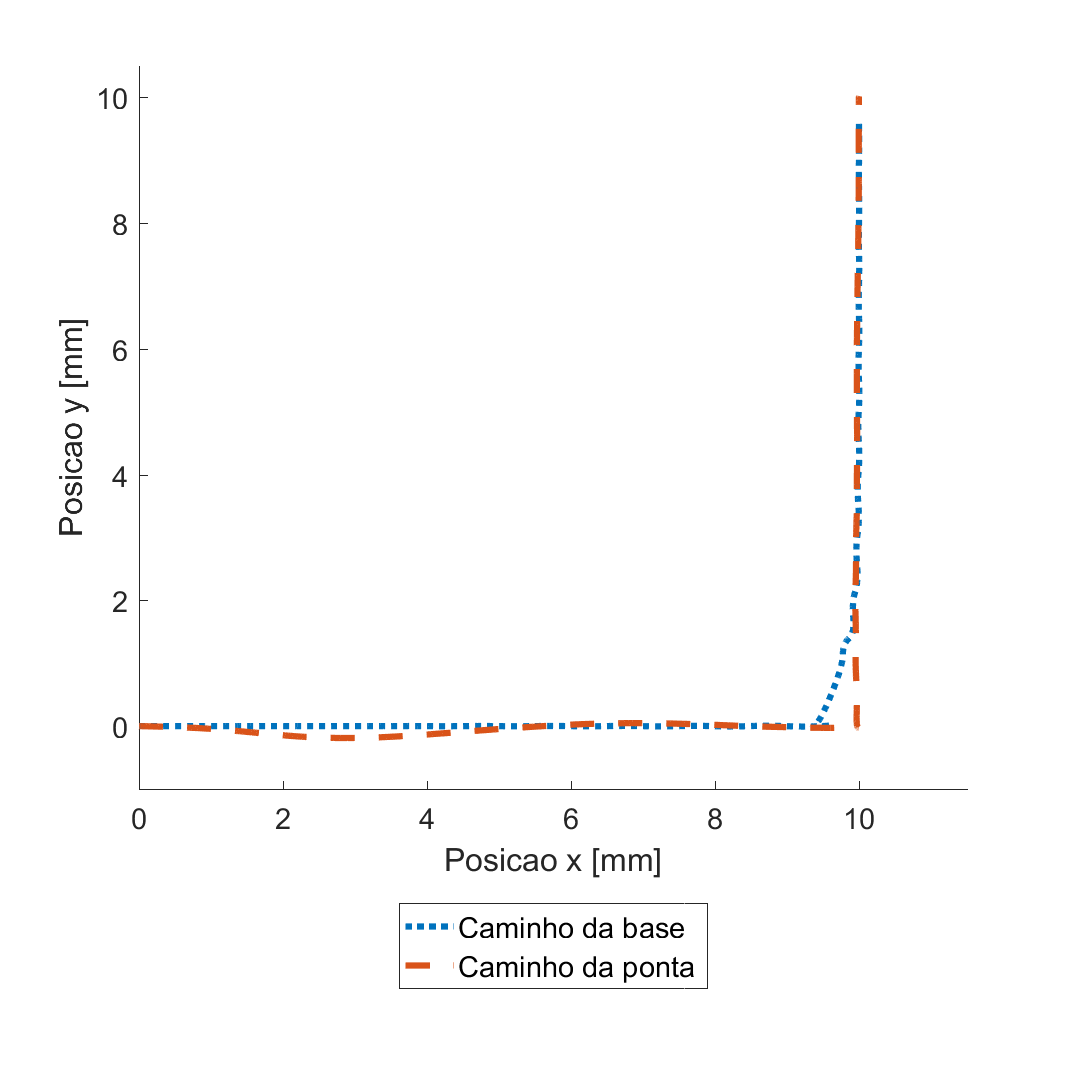
\includegraphics[width=0.47\textwidth]{Sim 3B_cam_c.png}
        \label{fig:3B_cam_c}
    }
    \hfill
    \subfigure[Detalhamento - Sem controle.]{
        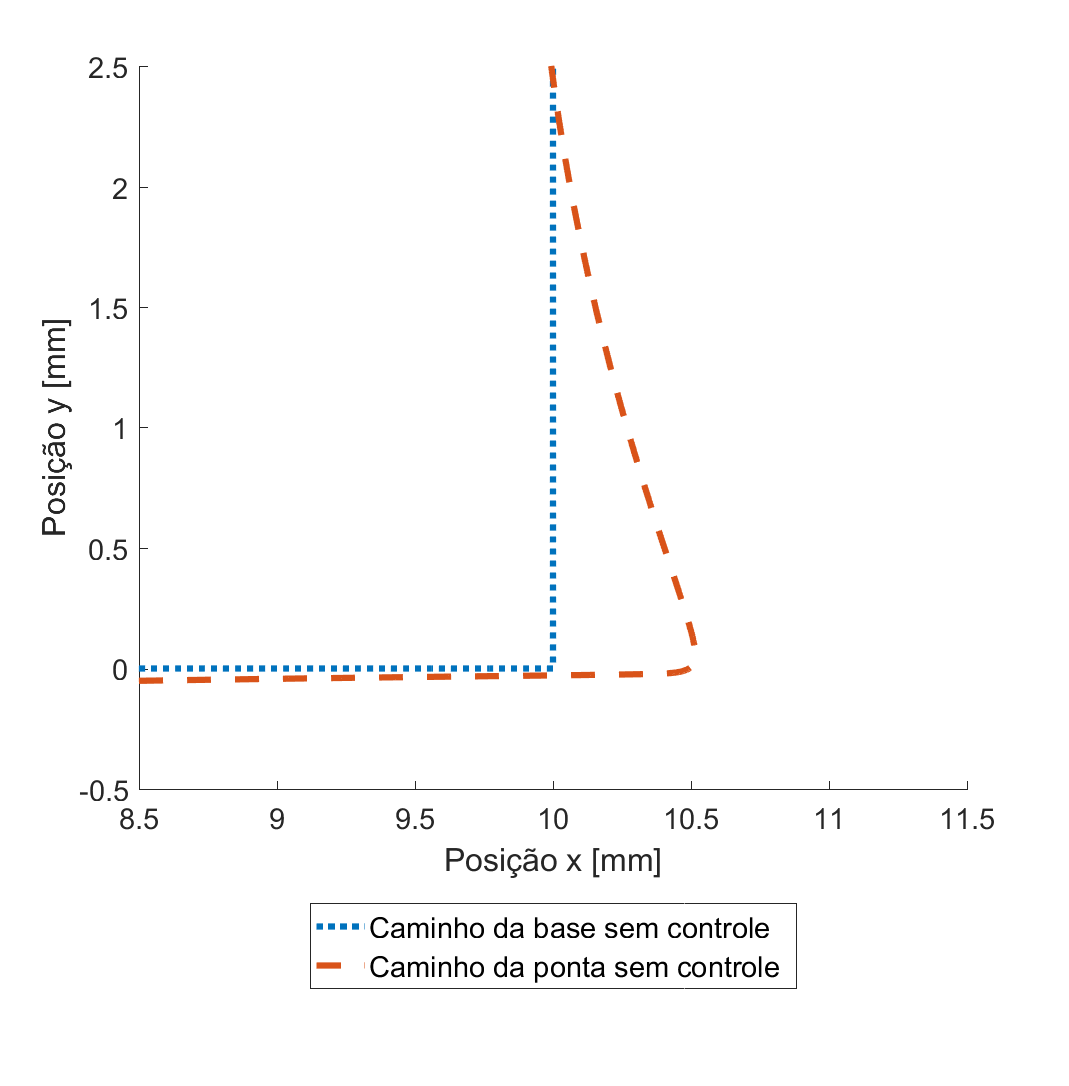
\includegraphics[width=0.47\textwidth]{Sim 3B_cam_s_zoom.png}
        \label{fig:3B_cam_s_zoom}
    }
    \hfill
    \subfigure[Detalhamento - Com controle.]{
        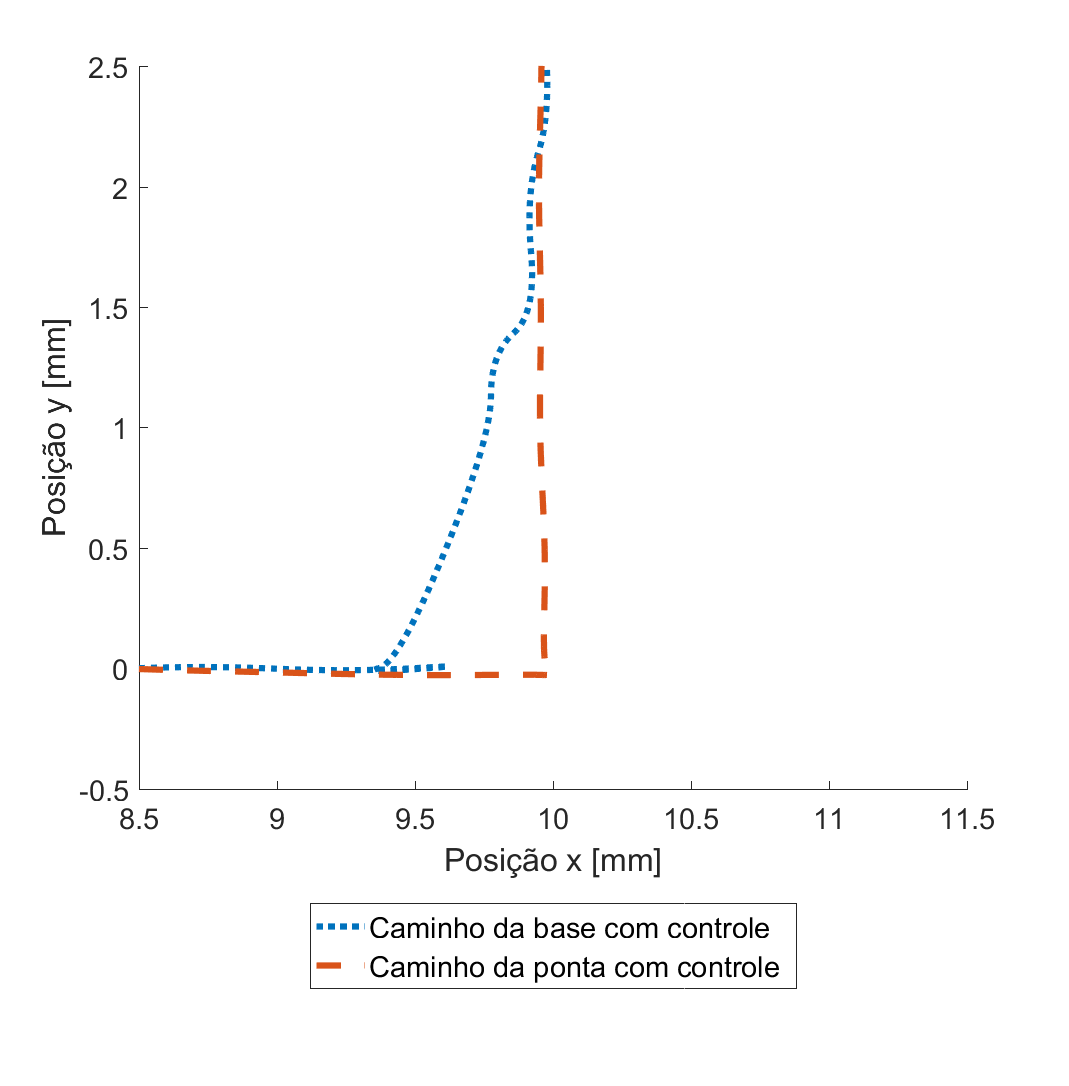
\includegraphics[width=0.47\textwidth]{Sim 3B_cam_c_zoom.png}
        \label{fig:3B_cam_c_zoom}
    }
    \caption{Caminhos da ponta e da base - Caso 3B.}
    \label{fig:3B_cam}
\end{figure}

% ------------------ Deslocamento A----------------

% fig:des
\begin{figure}[H]
    \centering
    \subfigure[Sem controle.]{
        \includegraphics[width=0.47\textwidth]{Sim 3A_des_s.png}
        \label{fig:3A_des_s}
    }
    \hfill
    \subfigure[Com controle.]{
        \includegraphics[width=0.47\textwidth]{Sim 3A_des_c.png}
        \label{fig:3A_des_c}
    }
    \caption{Deslocamentos da ponta e da base - Caso 3A.}
    \label{fig:3A_des}
\end{figure}

% ------------------ Deslocamento B----------------

% fig:des
\begin{figure}[H]
    \centering
    \subfigure[Sem controle.]{
        \includegraphics[width=0.47\textwidth]{Sim 3B_des_s.png}
        \label{fig:3B_des_s}
    }
    \hfill
    \subfigure[Com controle.]{
        \includegraphics[width=0.47\textwidth]{Sim 3B_des_c.png}
        \label{fig:3B_des_c}
    }
    \caption{Deslocamentos da ponta e da base - Caso 3B.}
    \label{fig:3B_des}
\end{figure}

% ------------------ Velocidades A ----------------
A variação da aceleração tem seu efeito primordial no perfil de velocidade criado na fase de geração de trajetória. É este parâmetro que dita as inclinações da curva de velocidade. Esse efeito pode ser observado nas Figuras \ref{fig:3A_vel_p} e \ref{fig:3B_vel_p}, onde é visível os ângulos menores e maiores entre os valores A (\(1000 mm/s^2\)) e B (\(10000 mm/s^2\)) respectivamente.

% fig:vel
\begin{figure}[H]
    \centering
    \subfigure[Sem controle.]{
        \includegraphics[width=0.47\textwidth]{Sim 3A_vel_s.png}
        \label{fig:3A_vel_s}
    }
    \hfill
    \subfigure[Com controle.]{
        \includegraphics[width=0.47\textwidth]{Sim 3A_vel_c.png}
        \label{fig:3A_vel_c}
    }
    \caption{Velocidades da ponta e da base - Caso 3A.}
    \label{fig:3A_vel}
\end{figure}

% ------------------ Velocidades B ----------------

% fig:vel
\begin{figure}[H]
    \centering
    \subfigure[Sem controle.]{
        \includegraphics[width=0.47\textwidth]{Sim 3B_vel_s.png}
        \label{fig:3B_vel_s}
    }
    \hfill
    \subfigure[Com controle.]{
        \includegraphics[width=0.47\textwidth]{Sim 3B_vel_c.png}
        \label{fig:3B_vel_c}
    }
    \caption{Velocidades da ponta e da base - Caso 3B.}
    \label{fig:3B_vel}
\end{figure}

% ------------------ end ----------------



\subsection{Caso 4 - Variação dos passos de tempo}

% ------------------ Caminho A ----------------
A variação dos passos de tempo utilizados na interpolação da trajetória criada na etapa de geração de trajetória possui o maior efeito na característica numérica do método de controle de trajetória. Este efeito pode ser observado na diferença de precisão entre as Figuras \ref{fig:4A_cam_p_s} e \ref{fig:4B_cam_p_s}, com seus respectivos passos de tempo \(0,01\) e \(0,0001\).

% fig:cam
\begin{figure}[H]
    \centering
    \subfigure[Sem controle.]{
        \includegraphics[width=0.47\textwidth]{Sim 4A_cam_s.png}
        \label{fig:4A_cam_s}
    }
    \hfill
    \subfigure[Com controle.]{
        \includegraphics[width=0.47\textwidth]{Sim 4A_cam_c.png}
        \label{fig:4A_cam_c}
    }
    \hfill
    \subfigure[Detalhamento - Sem controle.]{
        \includegraphics[width=0.47\textwidth]{Sim 4A_cam_s_zoom.png}
        \label{fig:4A_cam_s_zoom}
    }
    \hfill
    \subfigure[Detalhamento - Com controle.]{
        \includegraphics[width=0.47\textwidth]{Sim 4A_cam_c_zoom.png}
        \label{fig:4A_cam_c_zoom}
    }
    \caption{Caminhos da ponta e da base - Caso 4A.}
    \label{fig:4A_cam}
\end{figure}


% ------------------ Caminho B ----------------

% fig:cam
\begin{figure}[H]
    \centering
    \subfigure[Sem controle.]{
        \includegraphics[width=0.47\textwidth]{Sim 4B_cam_s.png}
        \label{fig:4B_cam_s}
    }
    \hfill
    \subfigure[Com controle.]{
        \includegraphics[width=0.47\textwidth]{Sim 4B_cam_c.png}
        \label{fig:4B_cam_c}
    }
    \hfill
    \subfigure[Detalhamento - Sem controle.]{
        \includegraphics[width=0.47\textwidth]{Sim 4B_cam_s_zoom.png}
        \label{fig:4B_cam_s_zoom}
    }
    \hfill
    \subfigure[Detalhamento - Com controle.]{
        \includegraphics[width=0.47\textwidth]{Sim 4B_cam_c_zoom.png}
        \label{fig:4B_cam_c_zoom}
    }
    \caption{Caminhos da ponta e da base - Caso 4B.}
    \label{fig:4B_cam}
\end{figure}

Além disso, outro grande efeito é no tempo de simulação, que se comparado às outras simulações realizadas, com uma média de 3 segundos, enquanto a execução da etapa de controle de trajetória com o passo de tempo mais fino este tempo chega a 93 segundos e o tempo do maior passo fica abaixo dos 0.5 segundos.

% ------------------ Deslocamento A----------------

% fig:des
\begin{figure}[H]
    \centering
    \subfigure[Sem controle.]{
        \includegraphics[width=0.47\textwidth]{Sim 4A_des_s.png}
        \label{fig:4A_des_s}
    }
    \hfill
    \subfigure[Com controle.]{
        \includegraphics[width=0.47\textwidth]{Sim 4A_des_c.png}
        \label{fig:4A_des_c}
    }
    \caption{Deslocamentos da ponta e da base - Caso 4A.}
    \label{fig:4A_des}
\end{figure}
% ------------------ Deslocamento B----------------

% fig:des
\begin{figure}[H]
    \centering
    \subfigure[Sem controle.]{
        \includegraphics[width=0.47\textwidth]{Sim 4B_des_s.png}
        \label{fig:4B_des_s}
    }
    \hfill
    \subfigure[Com controle.]{
        \includegraphics[width=0.47\textwidth]{Sim 4B_des_c.png}
        \label{fig:4B_des_c}
    }
    \caption{Deslocamentos da ponta e da base - Caso 4B.}
    \label{fig:4B_des}
\end{figure}
% ------------------ Velocidades A ----------------

% fig:vel
\begin{figure}[H]
    \centering
    \subfigure[Sem controle.]{
        \includegraphics[width=0.47\textwidth]{Sim 4A_vel_s.png}
        \label{fig:4A_vel_s}
    }
    \hfill
    \subfigure[Com controle.]{
        \includegraphics[width=0.47\textwidth]{Sim 4A_vel_c.png}
        \label{fig:4A_vel_c}
    }
    \caption{Velocidades da ponta e da base - Caso 4A.}
    \label{fig:4A_vel}
\end{figure}
% ------------------ Velocidades B ----------------

% fig:vel
\begin{figure}[H]
    \centering
    \subfigure[Sem controle.]{
        \includegraphics[width=0.47\textwidth]{Sim 4B_vel_s.png}
        \label{fig:4B_vel_s}
    }
    \hfill
    \subfigure[Com controle.]{
        \includegraphics[width=0.47\textwidth]{Sim 4B_vel_c.png}
        \label{fig:4B_vel_c}
    }
    \caption{Velocidades da ponta e da base - Caso 4B.}
    \label{fig:4B_vel}
\end{figure}
% ------------------ end ----------------

\subsection{Caso 5 - Variação da velocidade}

% ------------------ Caminho A ----------------

% fig:cam
\begin{figure}[H]
    \centering
    \subfigure[Sem controle.]{
        \includegraphics[width=0.47\textwidth]{Sim 5A_cam_s.png}
        \label{fig:5A_cam_s}
    }
    \hfill
    \subfigure[Com controle.]{
        \includegraphics[width=0.47\textwidth]{Sim 5A_cam_c.png}
        \label{fig:5A_cam_c}
    }
    \hfill
    \subfigure[Detalhamento - Sem controle.]{
        \includegraphics[width=0.47\textwidth]{Sim 5A_cam_s_zoom.png}
        \label{fig:5A_cam_s_zoom}
    }
    \hfill
    \subfigure[Detalhamento - Com controle.]{
        \includegraphics[width=0.47\textwidth]{Sim 5A_cam_c_zoom.png}
        \label{fig:5A_cam_c_zoom}
    }
    \caption{Caminhos da ponta e da base - Caso 5A.}
    \label{fig:5A_cam}
\end{figure}

% ------------------ Caminho B ----------------

% fig:cam
\begin{figure}[H]
    \centering
    \subfigure[Sem controle.]{
        \includegraphics[width=0.47\textwidth]{Sim 5B_cam_s.png}
        \label{fig:5B_cam_s}
    }
    \hfill
    \subfigure[Com controle.]{
        \includegraphics[width=0.47\textwidth]{Sim 5B_cam_c.png}
        \label{fig:5B_cam_c}
    }
    \hfill
    \subfigure[Detalhamento - Sem controle.]{
        \includegraphics[width=0.47\textwidth]{Sim 5B_cam_s_zoom.png}
        \label{fig:5B_cam_s_zoom}
    }
    \hfill
    \subfigure[Detalhamento - Com controle.]{
        \includegraphics[width=0.47\textwidth]{Sim 5B_cam_c_zoom.png}
        \label{fig:5B_cam_c_zoom}
    }
    \caption{Caminhos da ponta e da base - Caso 5B.}
    \label{fig:5B_cam}
\end{figure}
% ------------------ Deslocamento A----------------

% fig:des
\begin{figure}[H]
    \centering
    \subfigure[Sem controle.]{
        \includegraphics[width=0.47\textwidth]{Sim 5A_des_s.png}
        \label{fig:5A_des_s}
    }
    \hfill
    \subfigure[Com controle.]{
        \includegraphics[width=0.47\textwidth]{Sim 5A_des_c.png}
        \label{fig:5A_des_c}
    }
    \caption{Deslocamentos da ponta e da base - Caso 5A.}
    \label{fig:5A_des}
\end{figure}
% ------------------ Deslocamento B----------------

% fig:des
\begin{figure}[H]
    \centering
    \subfigure[Sem controle.]{
        \includegraphics[width=0.47\textwidth]{Sim 5B_des_s.png}
        \label{fig:5B_des_s}
    }
    \hfill
    \subfigure[Com controle.]{
        \includegraphics[width=0.47\textwidth]{Sim 5B_des_c.png}
        \label{fig:5B_des_c}
    }
    \caption{Deslocamentos da ponta e da base - Caso 5B.}
    \label{fig:5B_des}
\end{figure}
% ------------------ Velocidades A ----------------

% fig:vel
\begin{figure}[H]
    \centering
    \subfigure[Sem controle.]{
        \includegraphics[width=0.47\textwidth]{Sim 5A_vel_s.png}
        \label{fig:5A_vel_s}
    }
    \hfill
    \subfigure[Com controle.]{
        \includegraphics[width=0.47\textwidth]{Sim 5A_vel_c.png}
        \label{fig:5A_vel_c}
    }
    \caption{Velocidades da ponta e da base - Caso 5A.}
    \label{fig:5A_vel}
\end{figure}
% ------------------ Velocidades B ----------------

% fig:vel
\begin{figure}[H]
    \centering
    \subfigure[Sem controle.]{
        \includegraphics[width=0.47\textwidth]{Sim 5B_vel_s.png}
        \label{fig:5B_vel_s}
    }
    \hfill
    \subfigure[Com controle.]{
        \includegraphics[width=0.47\textwidth]{Sim 5B_vel_c.png}
        \label{fig:5B_vel_c}
    }
    \caption{Velocidades da ponta e da base - Caso 5B.}
    \label{fig:5B_vel}
\end{figure}
% ------------------ end ----------------

Os resultados da variação da velocidade desejada, definida junto aos movimentos do Gcode, possuem características muito semelhantes às variações no parâmetro da aceleração. De maneira que maiores velocidades desejadas resulta em menores tempo de impressão e maiores desvios do caminho, enquanto que para menores velocidades o oposto é verdade. Além disso, o controle de trajetória oferece analogamente à discussão da variação da aceleração, uma balança mais favorável à maiores velocidades desejadas, por meio de uma redução maior nos desvios de caminho.

\section{Discussão Integrada dos Resultados}
Realizadas as simulações com a variação dos parâmetros do método proposto no presente trabalho, ressalta-se a relação entre a frequência natural e o passo de tempo. Tal relação é muitas vezes discutida na literatura, se tratando de amostragem de sinais. É observado nestes resultados também, a relação entre a precisão alcançada e a proporcionalidade entre o passo de tempo e a frequência natural. Essa característica vem a tona ao se analisar o intervalo de tempo entre as oscilações e o passo de tempo. Onde um passo de tempo maior do que o período de oscilação, resulta em uma perda grande de informação e compromete a representatividade da curva discretizada. Sendo ideal um ajuste do passo de tempo dada a frequência natural conhecida do sistema.

A respeito dos demais parâmetros, estes se demonstraram mais independentes. Sendo os parâmetros de aceleração e velocidade desejada com efeitos finais similares.

\subsection{Considerações futuras}
Como comentado anteriormente, nota-se um grande aumento do tempo de execução da etapa de controle de trajetória para vetores maiores e por consequência para passos de tempo mais finos. Entretanto, muitas vezes os passos de tempo mais finos são necessários para se manter um nível de precisão do método aceitável. Uma abordagem a ser explorada para minimizar os tempos de simulação é a realização do controle de trajetória em etapas. Utilizando os resultados da trajetória da base de execuções com passos de tempo mais grosseiros como chute inicial para execuções com passos de tempo mais finos. Possivelmente reduzindo o tempo de execução final.

Outra ideia a ser explorada é a sobreposição de algoritmos. Onde
a dinâmica de um sistema, utilizando um primeiro método de controle de trajetória, ser aferida para fornecer parâmetros para um segundo método. Por exemplo, a aplicação da metodologia proposta neste trabalho, junto da aferição das características dinâmicas deste conjunto, impressora 3D e algoritmo de controle, através de um acelerômetro para assim aplicar em um segundo método como \textit{Input Shaping}.

Além disso, um ajuste do modelo dinâmico da impressora de forma espacial, pode favorecer métodos iterativos, também característico na metodologia aqui desenvolvida. Através da habilidade de descrever um sistema dinâmico mais complexo, a partir de um conjunto de sistemas dinâmicos mais simples sem que exista um comprometimento grande do custo computacional.


